\documentclass[../../../Bachelorarbeit.tex]{subfiles}
\begin{document}

\subsection{Implementationsphase} \label{implementation}
In diesem Unterkapitel findet sich die Dokumentation der Implementation sämtlicher Modelle aus der Projektierungsphase wieder. Zunächst wird im \autoref{Hardwareimp} die Montage der Laboranlage kurz dargestellt. Dazu wird aus der Konfiguratorskizze unter Berüchsichtigung der Maße des Laborraumes und der entsprechenden Anforderungen an den Aufbau des Positioniersystems die Anlage aufgebaut. Nachdem alle Gehäuseelemente an der Wand und dem Boden verankert sind können die Steuerungskomponenten, die Aktuatoren und die Sensoren an diesen befestigt werden. Weiterhin umfasst der nachfolgende Abschnitt die Verdrahtung der elektrischen Komponenten nach entwickeltem Stromlaufplan und der Netzwerkdarstellung aus dem \autoref{Stromlaufplan}.\\
Im zweiten Unterabschnitt (\autoref{Softwareimp}) wird die Implementation der modellierten Diagramme zur Steuerungssoftware vorgenommen. Da durch die Wahl der Steuerung (Logic Motion Controller von Schneider Electric), wie bereits in der Anforderungsanalyse festgestellt, die Umgebung zur Programmierung der Systemsoftware festgelegt ist, besteht die Möglichkeit Templates aus dieser zu nutzen, welche den Softwareentwicklungsprozess vereinfachen. Der Unterabschnitt zur Software-Implementation behandelt somit die schrittweise Darstellung der Umsetzung der Automatisierungssoftware aus dem von Schneider Electric bereitgestellten \textit{Motion Template Full}.

\subsubsection{Hardware-Implementation} \label{Hardwareimp}
Für die Umsetzung der Hardware wird die Kofiguratorgrafik aus der Konzeptphase wird aufgegriffen und gilt als Grundlage für die reale Umsetzung der Hardwarebereiche des Systems. Da im Konfigurator bereits die Kernanforderungen an die Systemhardware berücksichtigt wurden, müssen beim Bau und der Montage des Gehäuses \bzw des Anlagengerüsts nur noch die nicht-funktionalen Anforderungen an dieses und den umliegenden Raum berücksichtigt werden.\\
Durch die Form und die Ausmaße des Laborraumes ergibt sich eine maximale Höhe des Gehäuses von 2230\si{\mm}. Die horizontale Ausdehnung der Anlage wird nicht durch den Raum begrenzt. Die Entscheidung wurde auf Grund von Subjektiven Anschaulichkeitskriterien getroffen. Resultat ist eine horizontale Ausdehnung der x-Achse von 2000\si{\mm}, was ungefähr der Gangbreite im Laborraum entspricht. Folglich ist der bewegliche Teil des Positioniersystems mittig zum Durchgang im Raum ausgerichtet. Sowohl rechts als auch links neben der Positioniereinheit ist ein bereich von jeweils 600\si{\mm} reserviert, in dem Ablagepositionen an der Wand befestigt weren können. Die rechte Seite der Anlagenkonstruktion besitzt zusätzlich noch ein weiteres Aluminium Profil, welches später benötigt wird, um den Schaltschrank und die Steuerungshardware am System zu fixieren. Nachfolgende Grafik zeigt das an der Laborraumwand montierte Anlagengerüst, an welches im nächsten Schritt die Steuerungshardware befestigt wird.

\begin{figure}[H]
    \centering
    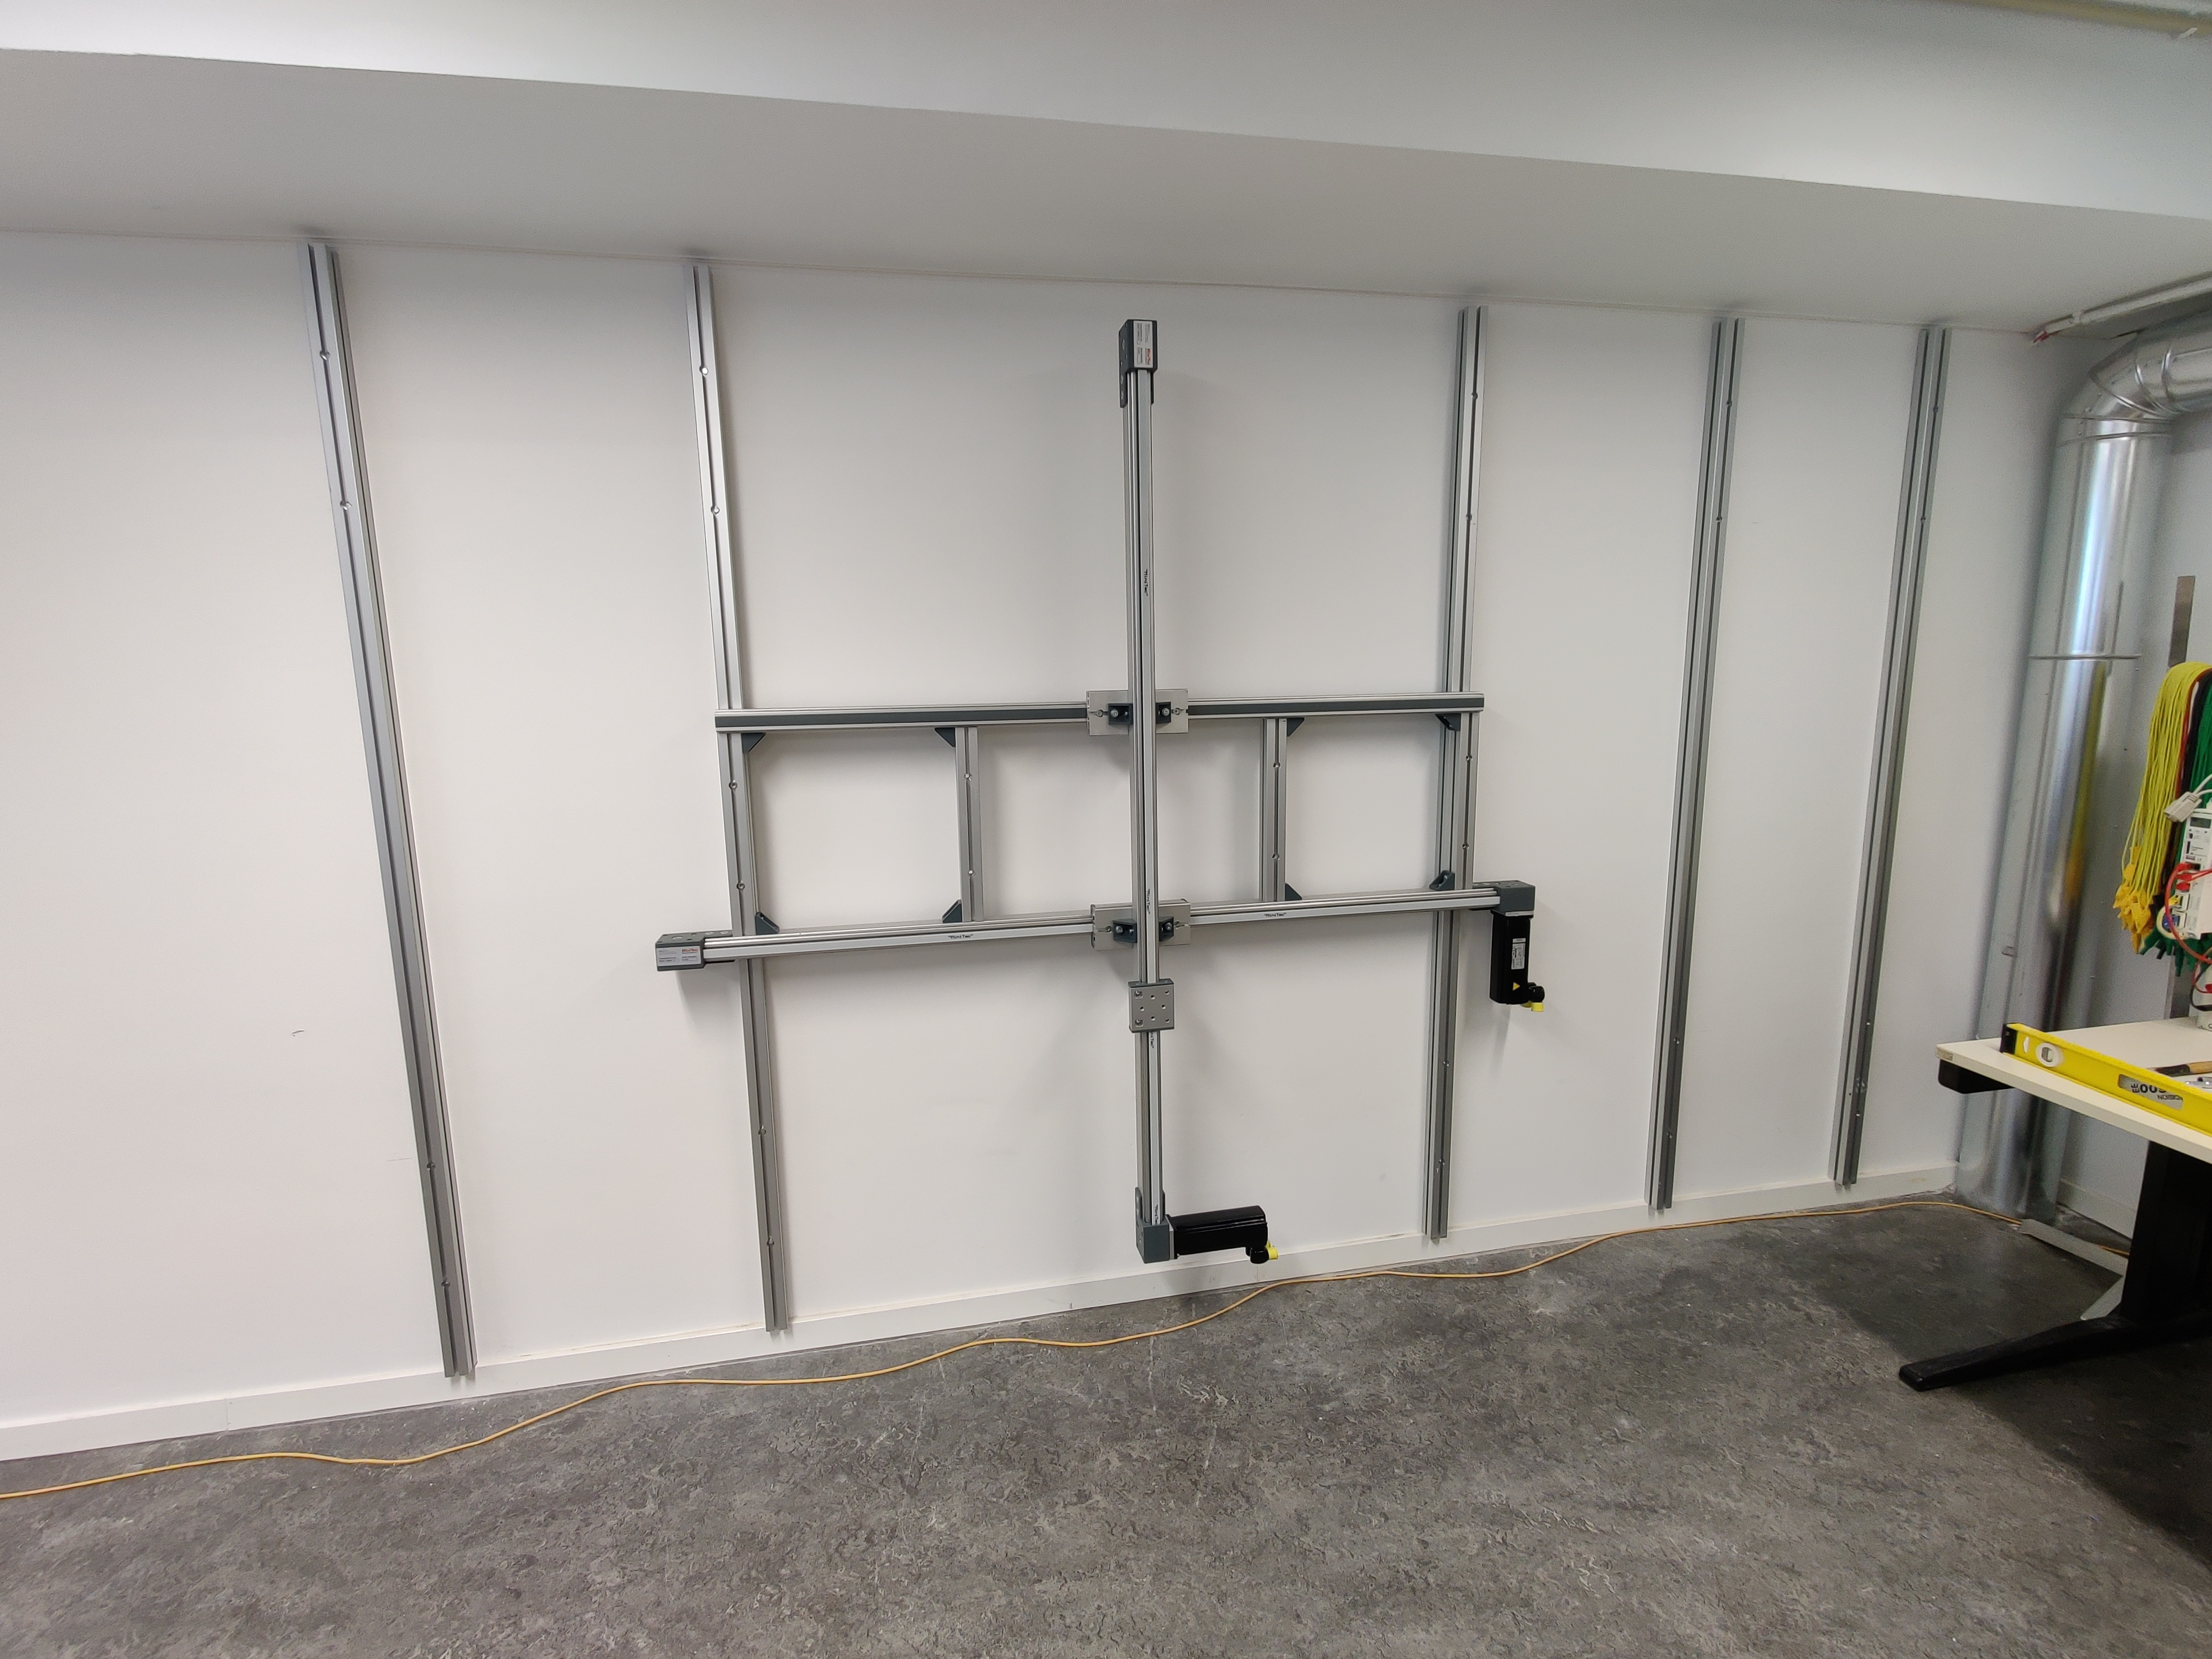
\includegraphics[width=0.7\textwidth]{Images/Anlagengeruest.jpg}
    \caption[Anlagengerüst]{Anlagengerüst des Gehäuses vom mehrachsigen Positioniersystem an der hinteren Laborwand im Raum G 422}
    \label{fig:my-img20}
\end{figure}

Im nächsten Schritt der Hardware-Implementation werden die Steuerung (LMC400) das Netzgerät (LXM 62P) und der Servoregler (LXM 62D) an Querverstrebungen der beiden rechten Profile verschraubt. Es gilt die Montageanleitung zu beachten.

\begin{figure}[H]
    \centering
    \begin{subfigure}[c]{0.42\textwidth}
        \centering
        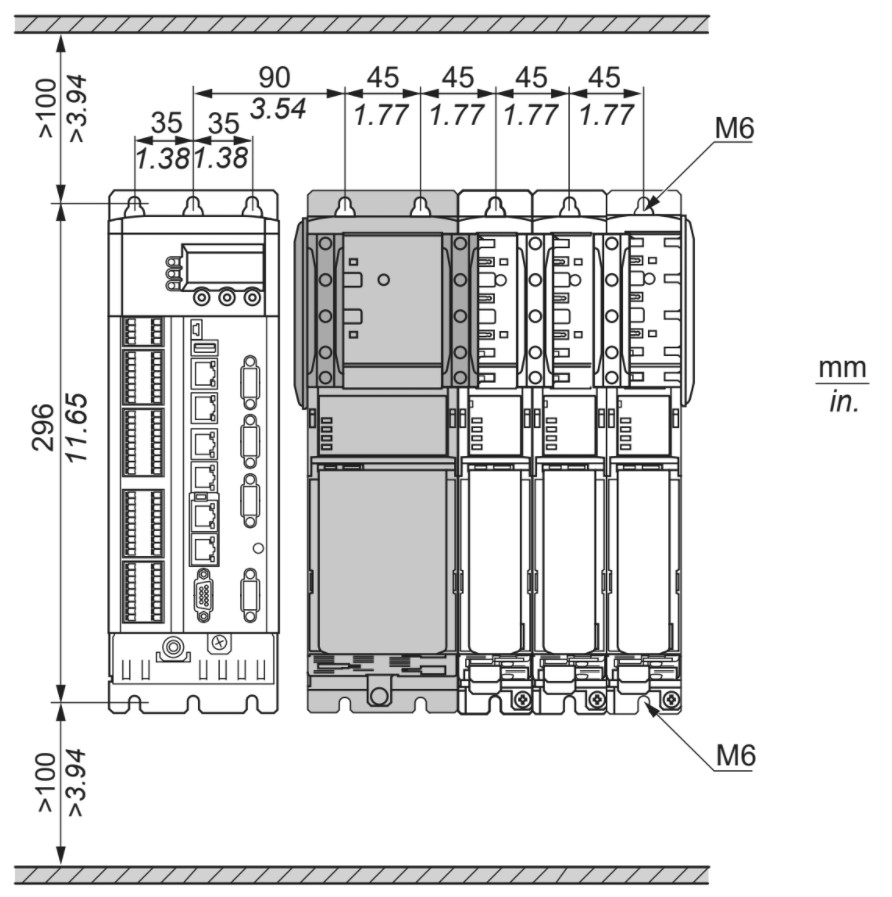
\includegraphics[width=0.9\textwidth]{Images/Steuerungshardwareinstallation.jpg}
    \end{subfigure}
    \begin{subfigure}[c]{0.42\textwidth}
        \centering
        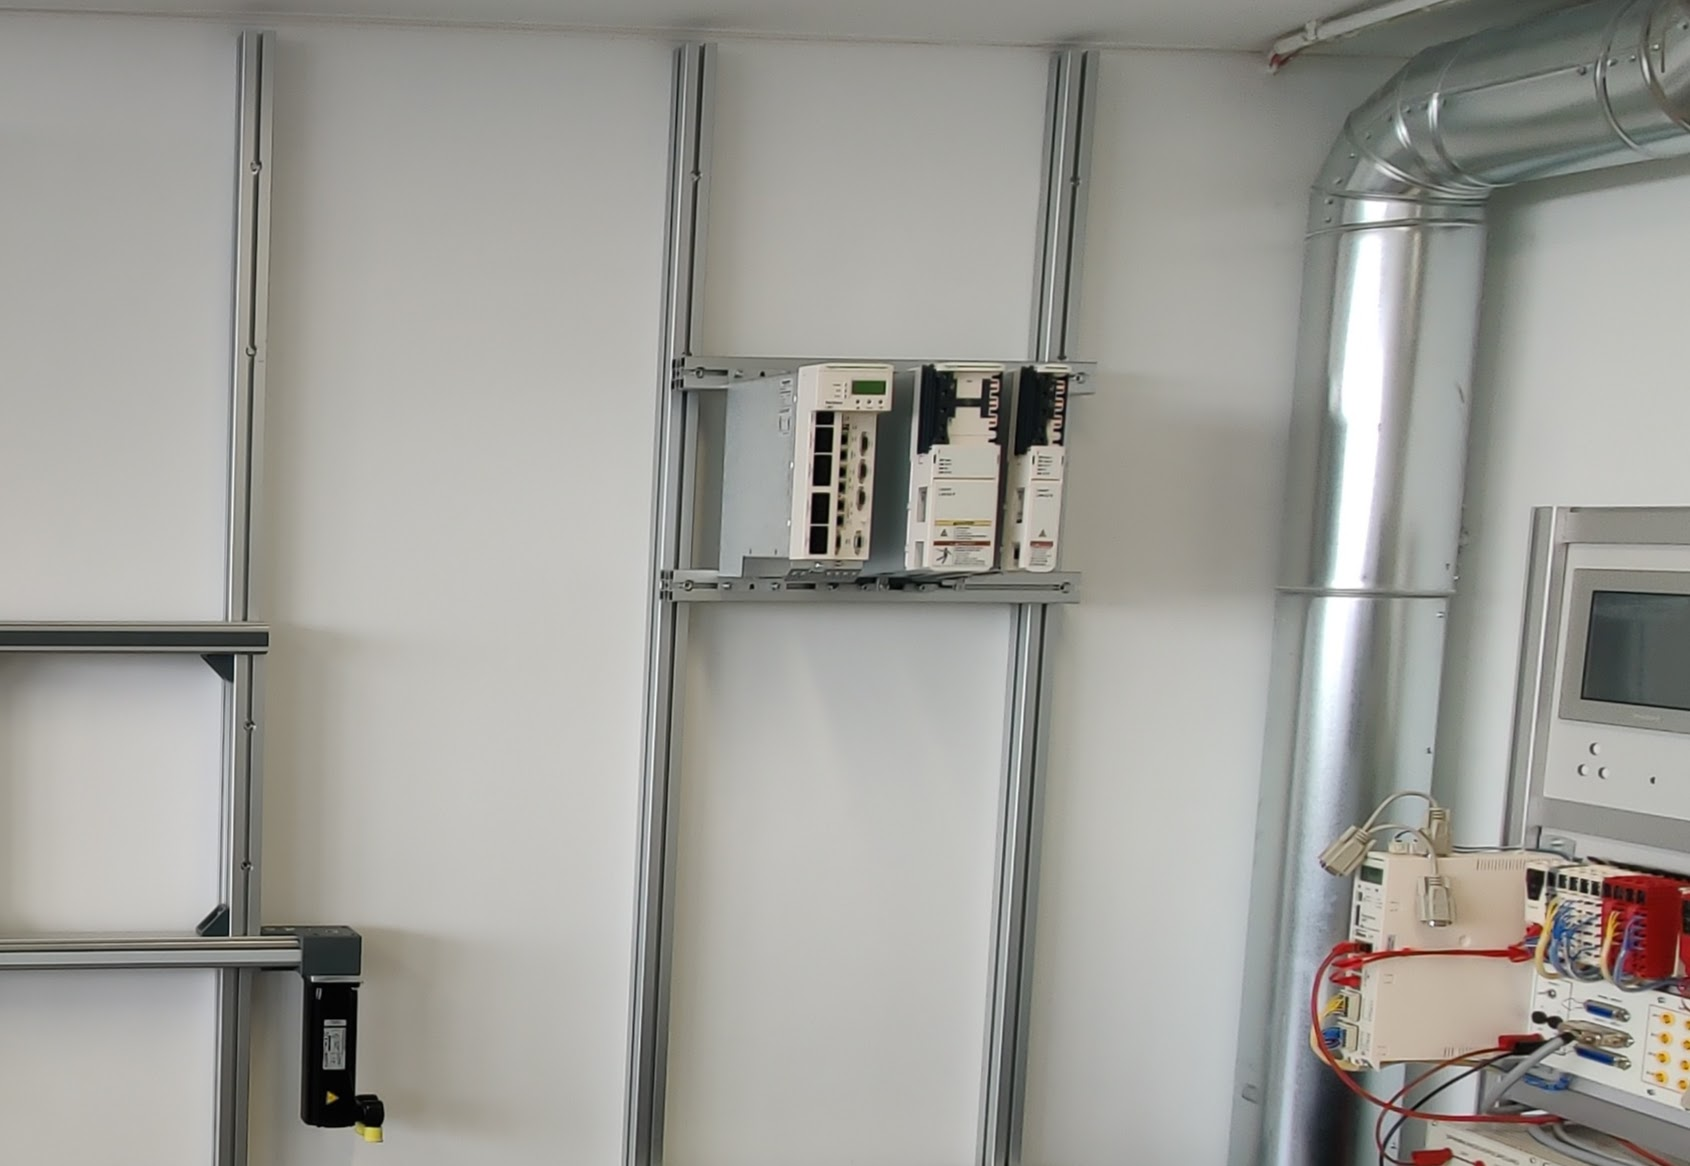
\includegraphics[width=0.9\textwidth]{Images/Steuerungshardware.jpg}
    \end{subfigure}
    \caption[Steuerungsinstallation]{Installation der Steuerungshardware am Gehäuseaufbau des Positioniersystems}
    \label{fig:my-img21}
\end{figure}

Bevor die in der Konfiguratorskizze aufgeführten Sensoren und Aktuatoren verbaut werden können, sind noch weitere Profile notwendig, um den Gehäusebau zu komplettieren. 500\si{\mm} von der Wand entfernt auf Höhe der äußeren Profile des Positionierbereiches werden zwei senkrechte Aluminiumstempel an Decke und Boden befestigt. Diese sind das vordere Ende des mehrachsigen Positioniersystems. Das Gehäusegerüst ist nun vollständig und umschließt den Berech, in dem Positionieraufgaben durchgeführt werden können mit der Laboranlage.\\
Zwischen den beiden linken Profilen und den beiden rechten Profilen werden Plexiglasscheiben angebracht, die das Hineingreifen in den Fahrbereich der Anlage von den Seiten verhindern sollen. An der Front wird ein Lichtvorhang bestehend aus Emitter und Receiver montiert. Dieser befindet sich auf der Innenseite an den zuletzt angebauten senkrechten Stempeln. Der Lichtvorhang dient ebenso wie die Plexiglasscheiben zum Schutz von Leib und Leben. Im Gegensatz zu den Scheiben erlaubt der Lichtvorhang jedoch im unbewegten Zustand des Systems das Eindringen von Personen in des Arbeitsbereich.\\
Folgende Grafik zeigt zu den soeben genannten Komponenten zusätzlich noch die in den Anforderungsanalyse ermittelten vier Endlagesensoren, die Servomotoren für x- und z-Achse, sowie E-Ketten zu den beweglichen Achsen.

\begin{figure}[H]
    \centering
    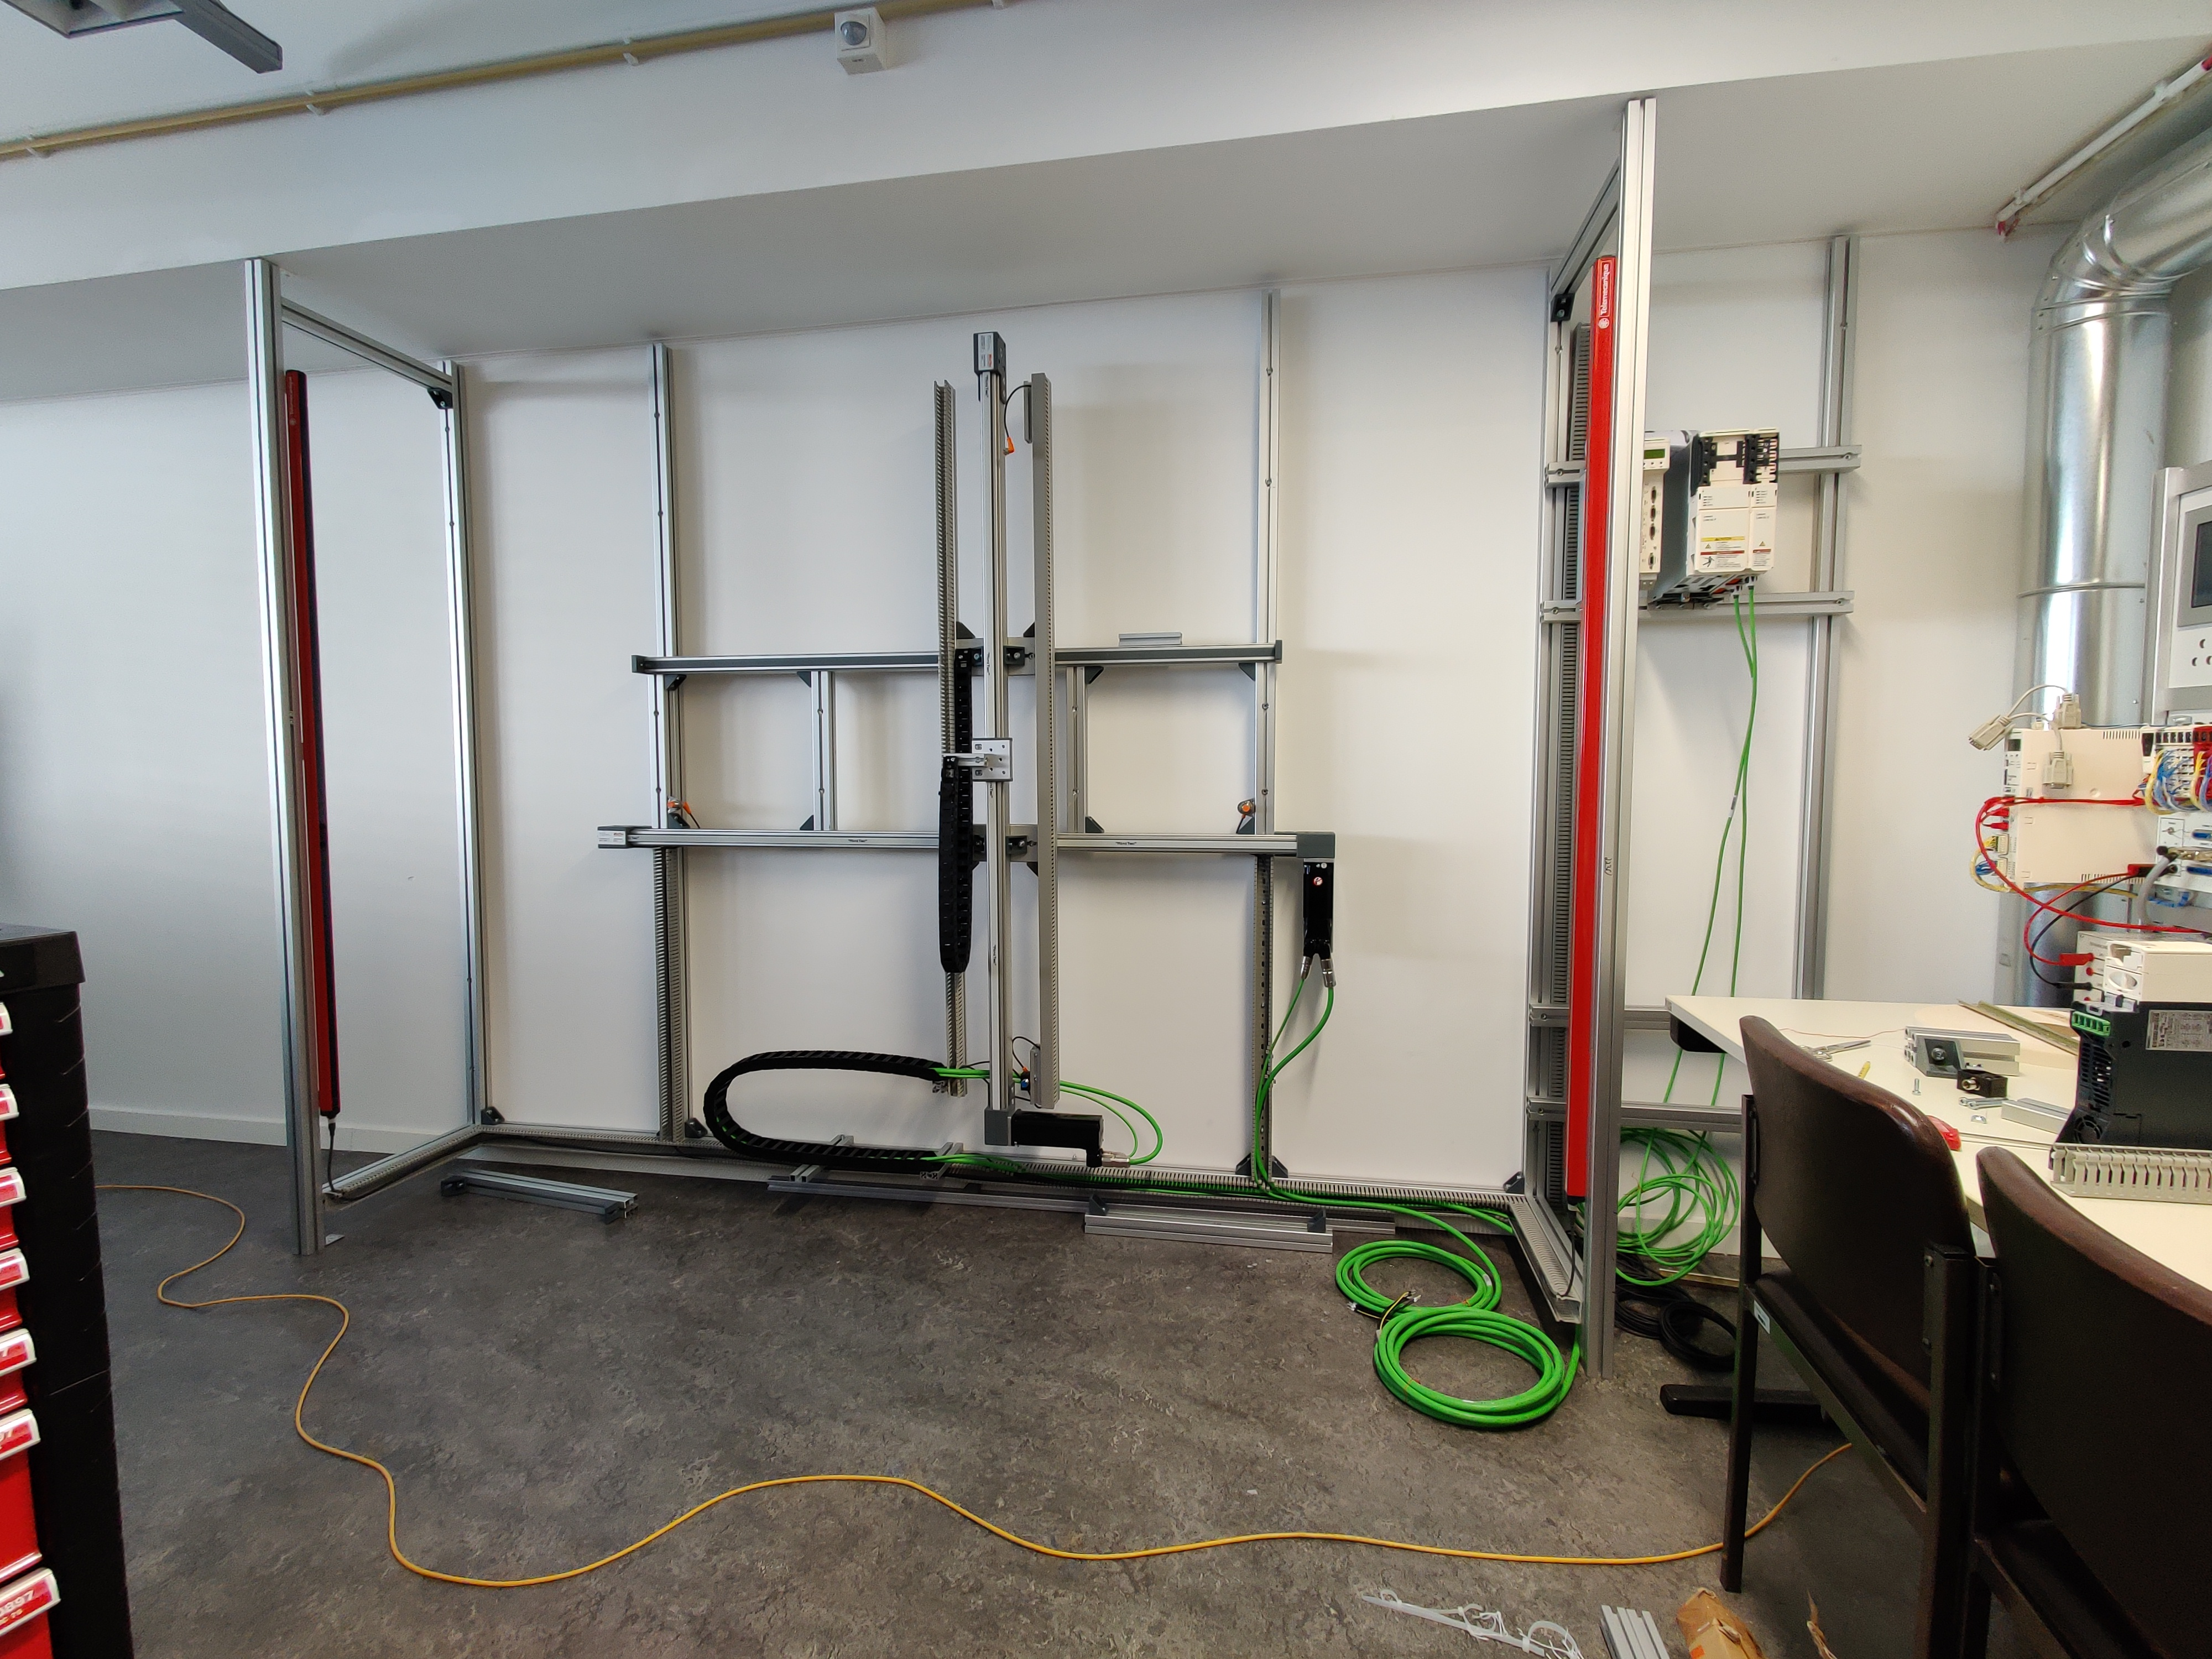
\includegraphics[width=0.7\textwidth]{Images/AktuatorenSensoren.jpg}
    \caption[Aktuator- und Sensorinstallation]{Installation von Sensoren und Aktuatoren des mehrachsigen Positioniersystems}
    \label{fig:my-img22}
\end{figure}

Der Schaltschrankeinbau und die Verdrahtung des Systems stellt den letzten Schritt in der Hardware-Implementierung dar. Als Schaltschrank wurde ein Modell der Firma Rittal gewählt. Die Breite des Schrankes ist durch den gewählten Aufbau bereits festgelegt und beträgt 600\si{\mm}. Aufgrund der Anzahl der Klemmen und dem Wunsch \acs{ea}-Module sowie weitere Steuerungskomponenten physisch von normalen Klemmen zu trennen, wurde entschieden eine Schaltschrankkonfiguration zu wählen, die in der Höhe zwei Hutschienen unterbringt. Die gewählte Schrankhöhe liegt deswegen bei 380\si{\mm}. Zuletzt muss die Tiefe des Schaltschranks ausreichend sein, um die tiefste Komponente, die im Schaltschrank verbaut werden soll, unterbringen zu können. Da bereits die kleinste verfügbare Variante des gewählten Schrankes diese Anforderung erfüllt, hat der zu verbauende Schaltschrank eine Tiefe von 210\si{\mm}.\\
Wie bereits angedeutet ist in der Grafik unten zu erkennen, dass die untere der beiden Hutschienen sämtliche Klemmen beherbergt inklusive der Absicherungen für die jeweilge Spannungsebene, so wie im Stromlaufplan geplant. An der Oberen Hutschiene befinden sich die Modicon TM5 \acs{ea}-Module, die als Erweiterung für die Ein- und Ausgänge des \acs{lmc} dienen. Die im Bild als rot gefärbte Komponente zu erkennende Steuerung, ist der Safety Logic Controller, der für die Berechnung der Sicherheitsfunktionen des Systems verantwortlich ist. Dazu besitzt dieser jeweils vier digitale Ein- und Ausgänge.\\
Rechts daneben auf der selben Schiene ist die Wago PFC 200 Steuerunge angebracht, welche mit Hilfe ihrer Energieklemme die Leistungsaufnahme des Systems messen soll.\\
Ganz Rechts auf der Hutschiene ist ein Ethernetswitch montiert, an welchen beide Steuerungen (LMC400 und Wago PFC 200) per Ethernetkabel angeschlossen sind. Durch den Einsatz des Switches führt nach Vertigstellung der verdrahtung nur ein Kabel zur Programmierung der beiden Steuerungen aus dem Schaltschrank heraus.\\
Weiterhin ist auf der rechten Schrankwand der Hauptschalter platziert. Über dieser aktiviert oder deaktiviert die Stromversorgung des Schaltschrankes und somit auch aller Systemkomponenten.\\
Die Verdrahtung erfolgt nach Stromlaufplan. Dieser beinhaltet auch die Kopplung der einzelnen Module aus der PacDrive3 Serie, die verbaut wurden (LMC400, LXM 62P, LXM 62D, Modicon TM5 Module, Modicon TM5 SLC100 Sicherheitsmodule). 

\begin{figure}[H]
    \centering
    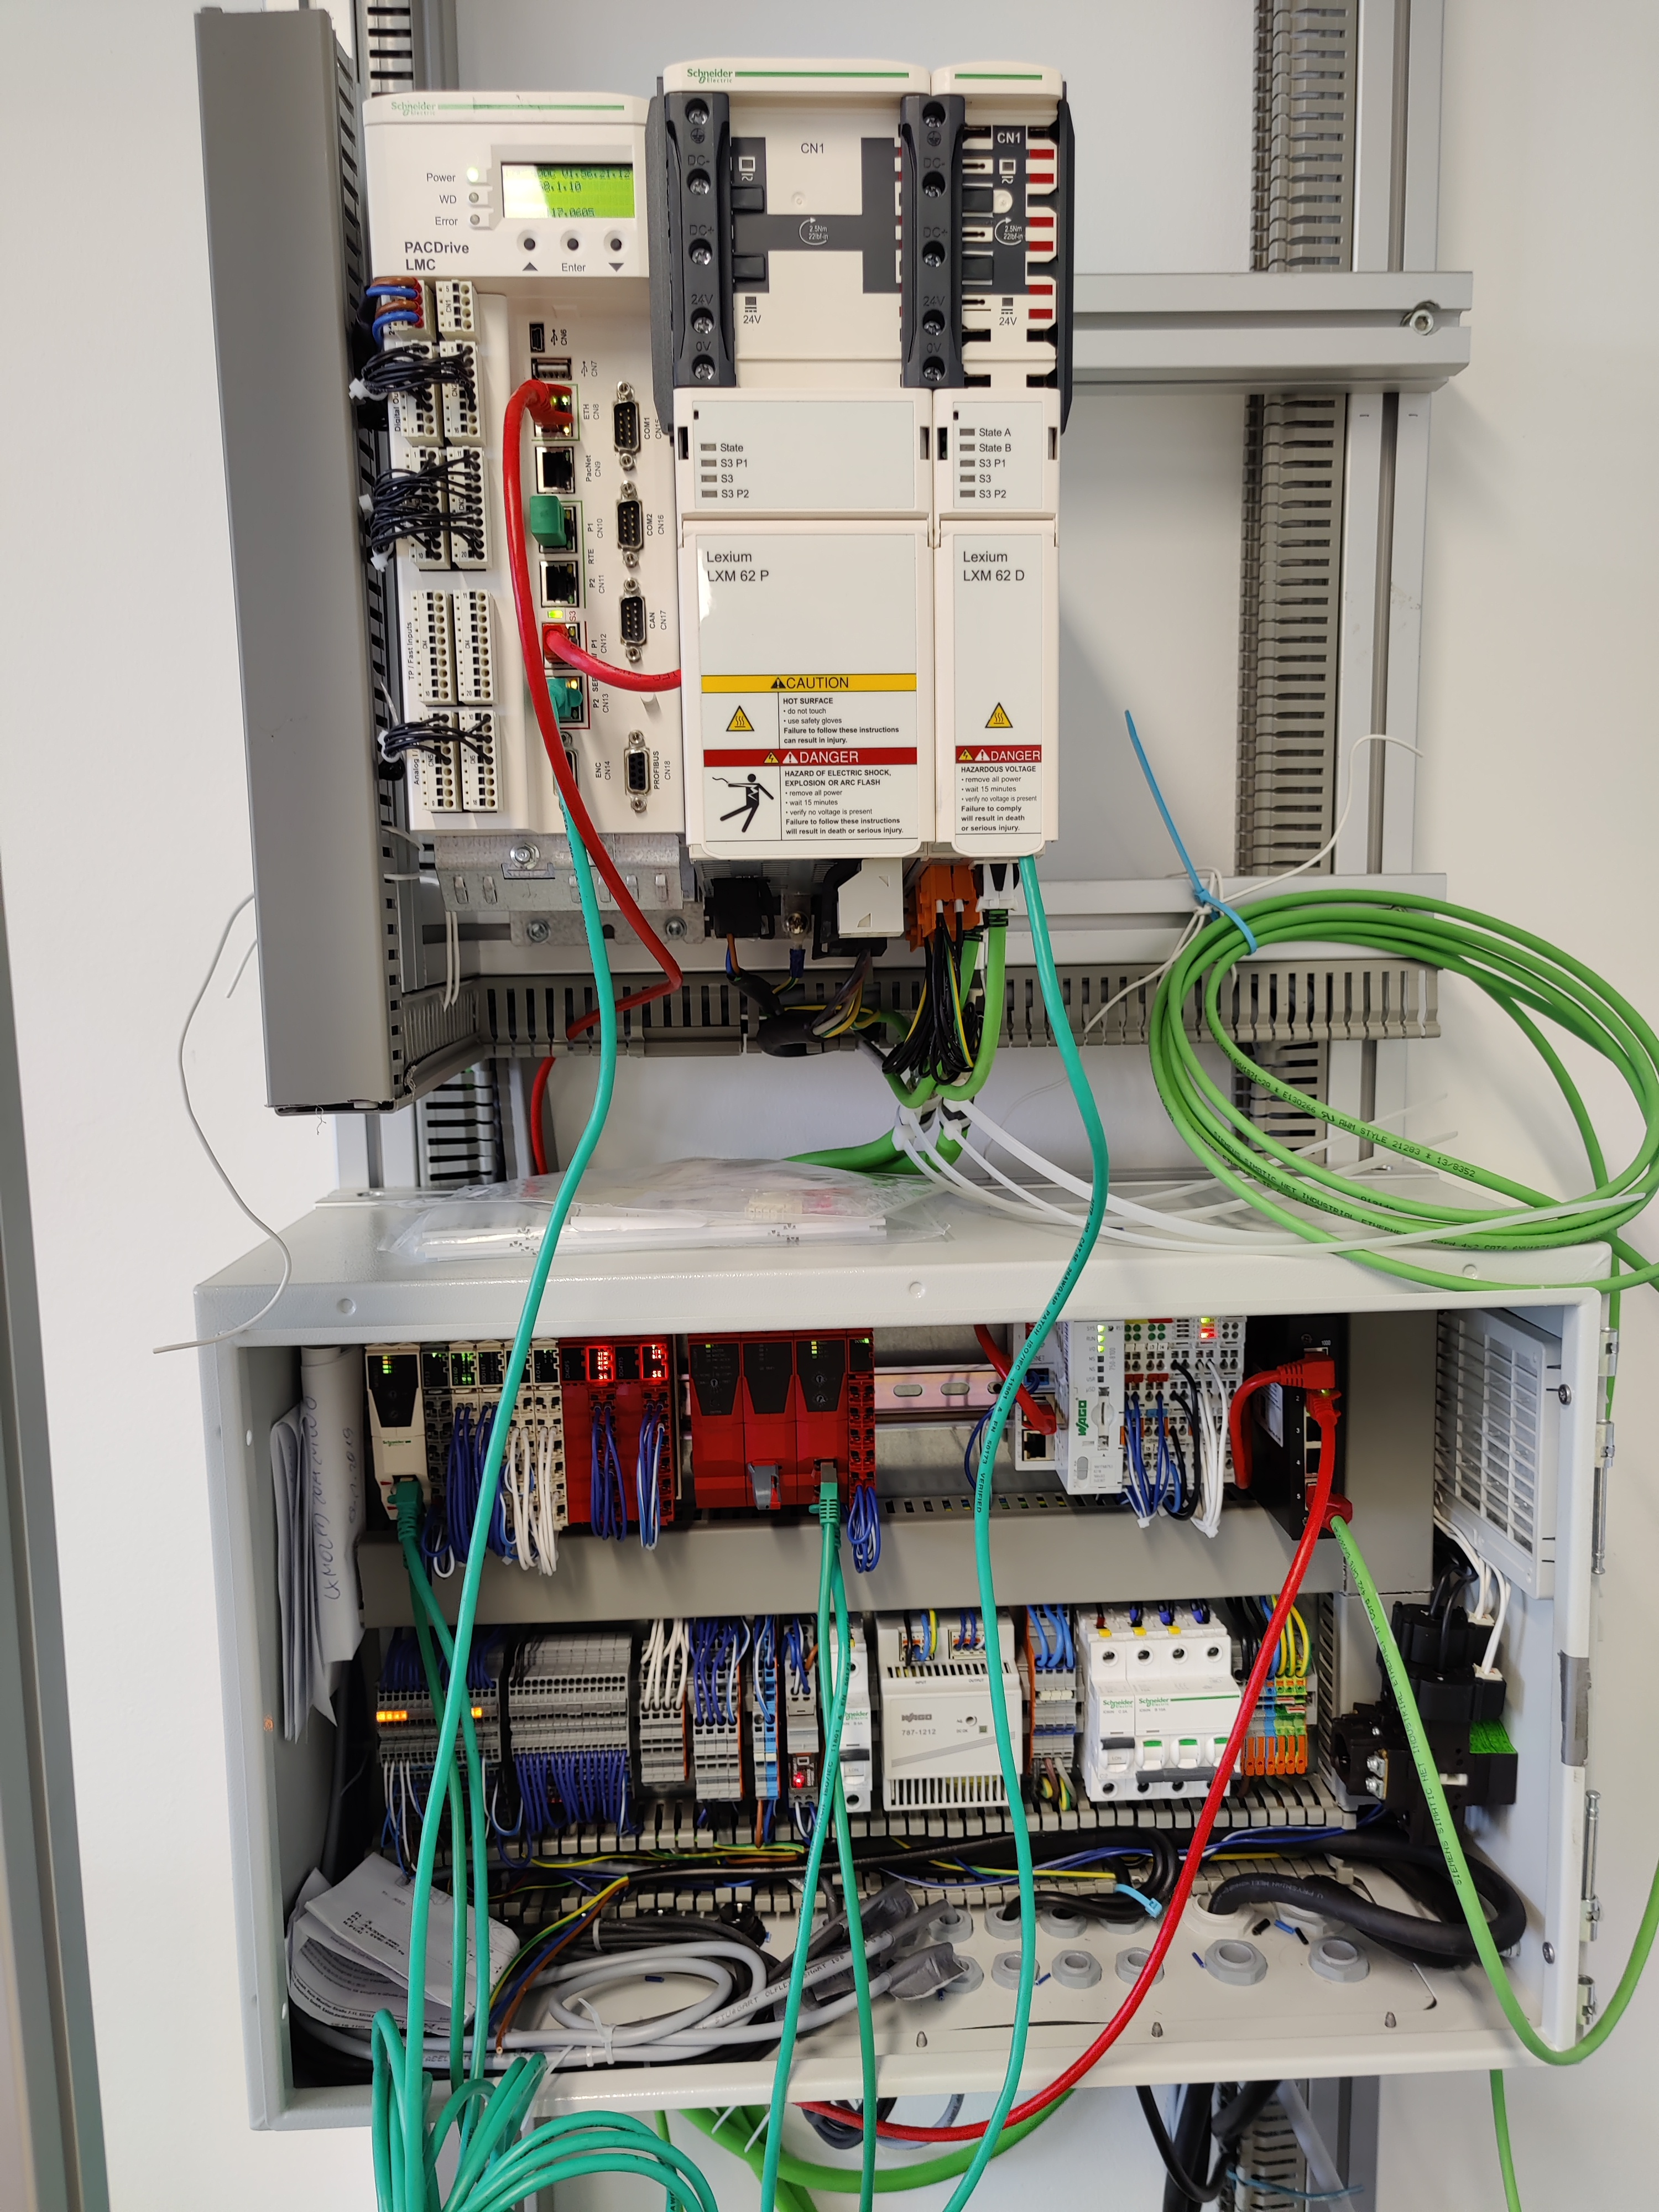
\includegraphics[width=0.66\textwidth]{Images/Schaltschrank.jpg}
    \caption[Schaltschrank]{Einbau und Verdrahtung des Schaltschranks}
    \label{fig:my-img23}
\end{figure}

% Schaltschrankfront Text + Bild !!!

\subsubsection{Software-Implementation} \label{Softwareimp}
In diesem Unterabschnitt wird die Realisierung der Automatisierungssoftware dokumentiert. Grundlegend soll aus der Modellierung der Software im vorhergegangenen Kapitel (Projektierung) das Programm für das mehrachsige Positioniersystem geschrieben werden. Wie bereits in der Einleitung zu diesem Unterkapitel erwähnt, resultiert die Wahl der Steuerungskoponenten, also konkret die Wahl Komponenten aus der PacDrive3 Serie von Schneider Electric auszuwählen, in dem Zwang mit der auf Codesys 3.5 basierten Entwicklungsumgebung Machine Expert zu arbeiten. Diese besitzt bereits mehrere Templateprojekte für verschiedene Anweundungsfälle. Die Firma Schneider Electric empfiehlt die Nutzung des jeweiligen Programmtemplates für den gewünschten Anwendungsfall. Grund dafür ist die Minimierung vom Programmieraufwand. Ziel soll es sein lediglich Konfigurationen an einem Modularen Template vorzunehmen, so dass dieses die eigenen Anforderungen erfüllt. \\
Begründet durch diese Aussagen wird zunächst davon ausgegangen, dass durch die Nutzung des \textit{Motion Template Full} mit überschaubarem Programmier- und Parametrieraufwand die Sammlung der eigenen Anforderungen an das Automatisierungsprogramm und dessen Funktionen erfüllt werden. Dies gilt im anschließenden Unterkapitel in den jeweiligen Testfällen zu bestätigen. \\
Zunächst findet eine schrittweise Auflistung zur Umsetzung der Steuerungssoftware aus dem bereitgestelltem Template statt. Diese unterteilt sich in folgende Vorgehensschritte:

\begin{itemize}
    \item Anlegen des Projektes
    \item Zuweisen der Ein- und Ausgänge der Steuerungen und deren Erweiterungsmodule (\eng Mapping)
    \item Parametrierung und Inbetriebnahme des Servoreglers für die x-Achse
    \item Parametrierung und Inbetriebnahme des Servoreglers für die z-Achse
    \item Parametrierung und Inbetriebnahme des Netzteils
    \item Implementation der funktionalen Sicherheit
\end{itemize}

Für das \textbf{Anlegen des Projektes} wird die Software Machine Expert Logic Builder auf den Rechnern des Labores benötigt. Alternativ kann auch die veraltete Software SoMachine Logic Builder genutzt werden. Soll von jedem PC aus das System Programmiert und zunächst auch gesteuert werden, so muss die Programmiersoftware vorhanden sein. Ist dies der Fall, so muss anschließend wie folgt vorgegangen werden:

\begin{enumerate}
    \item \textit{LogigBuilder} Programm am Laborcomputer starten
    \item Neues Projekt aus Projektvorlage \textit{MotionTemplateFull} für LMC300/400/402/600/800 anlegen
    \item Im Projektbaum oben links Doppelklick auf \textit{LMC\_PacDrive}
    \item Anschließend im Reiter \textit{Steuerungsauswahl} den LMC400c auswählen (vorher sichergehen, dass der Controller eingeschaltet ist, sonst kann dieser nicht gefunden werden)
    \item Im Projektbaum unter \textit{Sercos\_Master (Sercos Master)} alle untergeordneten Geräte markieren und anschließen entfernen
    \item Etwas tiefer im Projektbaum Doppelklick auf \textit{Geräteaddressierung}
    \item Im neu geöffneten Fenster oben rechts den Button \textit{Sercos Scan starten} drücken
    \item Es erscheinen neue tabellarisch angeordnete Einträge in der Mitte des Fensters (Einträge sind rot eingefärbt)
    \item Unten rechts im offenen Fenster auf \textit{Geräteparameter übernehmen} klicken (Alle vorhandenen Einträge sollten die Farbe zu grün wechseln)
    \item Den \textit{IEC Bezeichner} des Powersupplies ändern zu \textit{PSM\_PowerSupply}
    \item Den \textit{IEC Bezeichner} des von Drive A und B ändern zu \textit{DRV\_Slave1} \bzw \\ \textit{DRV\_Slave2}
    \item Oben links im offenen Fenster über Kombobox drei neue LXM62DxS hinzufügen
    \item \textit{IEC Bezeichner} des ersten neuen Eintrages auf \textit{DRV\_Master} ändern (Wichtig: Gerät sollte auf virtuell eingestellt sein)
    \item \textit{IEC Bezeichner} der beiden anderen Einträge ändern zu \textit{DRV\_Slave3} \bzw \\ \textit{DRV\_Slave4} (Wichtig: Geräte sollte auf virtuell eingestellt sein)
\end{enumerate}

\begin{figure}[H]
    \centering
    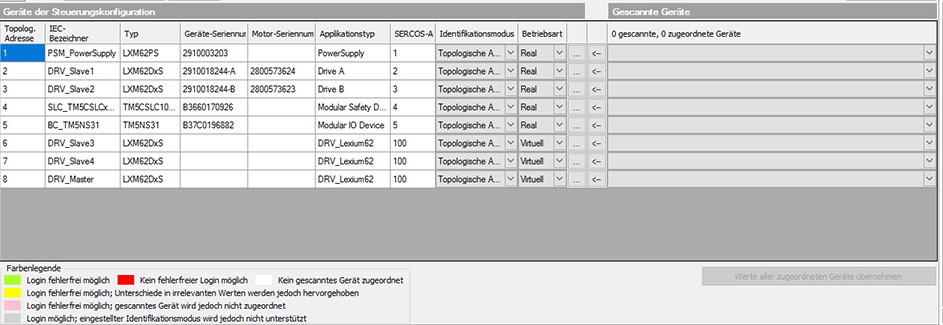
\includegraphics[width=0.66\textwidth]{Images/Sercos.png}
    \caption[Geräteaddressierung]{Geräteaddressierung der SERCOS III Busteilnehmer}
    \label{fig:my-img24}
\end{figure}

Um die anliegenden Sensor- und Eingabegerätesignale an den SPS Eingängen, sowie die Aktuatoren und Indikatoren an den SPS Ausgängen nutzen zu können, müssen den Hardwareaddressen im Programm Variablen zugewiesen werden (\eng \textbf{Mapping}). Damit alle \acs{ea}-Variablen an einem Ort als auch global im gesamten Programm verfügbar sind, sollte eine Globale Variablenliste angelegt werden, in der alle Variablen eingetragen werden können. Folgendes Bild zeigt die Globale Variablenliste für die Ein- und Ausgänge des mehrachsigen Positioniersystems.\\

\begin{figure}[H]
    \centering
    \begin{subfigure}[c]{0.42\textwidth}
        \centering
        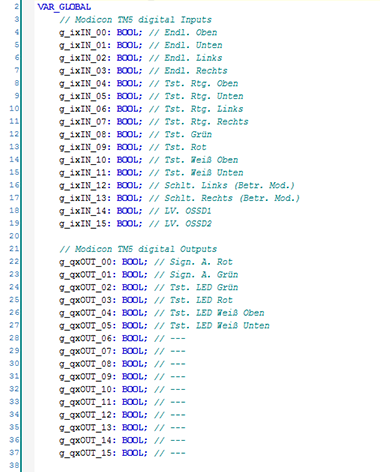
\includegraphics[width=0.9\textwidth]{Images/GVL1.png}
    \end{subfigure}
    \begin{subfigure}[c]{0.42\textwidth}
        \centering
        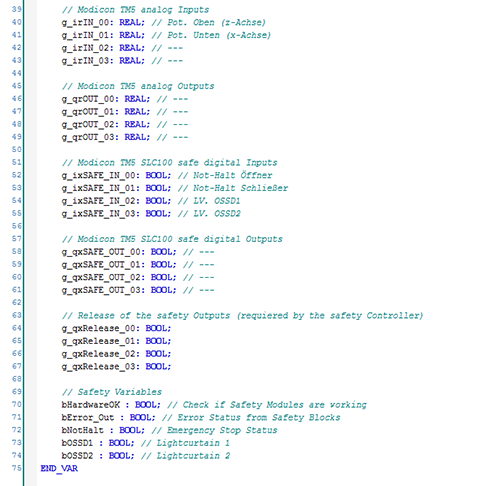
\includegraphics[width=0.9\textwidth]{Images/GVL2.png}
    \end{subfigure}
    \caption[Globale Variablenliste]{Globale Variablenliste der \acs{ea}-Variablen}
    \label{fig:my-img25}
\end{figure}

Nachfolgend wird das Mapping schrittweise für die Ein- und Ausgangsmodule der mit dem LMC verbundenen Modicon TM5 Geräte vorgenommen. Bei den zuzuordnenden Variablen handelt es sich um die im Datenmodell aufgelisteten Variablen. Dieses dient somit als Grundlage für die Zuweisung der Ein- und Ausgänge.

\begin{itemize}
    % Digitale Eingänge
    \item Zuweisung der digitalen Eingänge des Modicon \textit{TM5SDI16D} Modul:
    \begin{enumerate}
        \item Im Gerätebaum öffnen der Geräteeinstellungen des Moduls unter \textit{Sercos\_Master (Sercos Master)} ->\small \textit{BC\_TM5NS31 (BC\_TM5NS31)} -> \textit{TM5SDI16D (TM5SDI16D)}
        \item \normalsize Öffnen des Reiters \textit{SERCOS III Module E/A-Abbild}
        \item \begin{minipage}[t]{\linewidth}
            \raggedright
            \adjustbox{valign=t}{%
                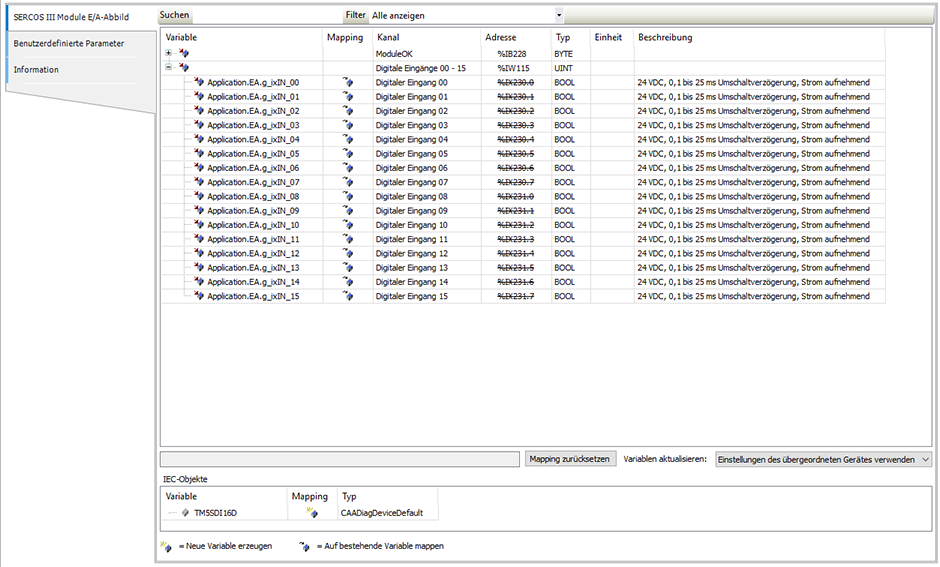
\includegraphics[width=.8\linewidth]{Images/TM5DI.PNG}%
            }
            \captionof{figure}{Zuweisung der digitalen Eingänge des \small TM5SDI16D \normalsize Moduls}
            \label{fig:my-img26}
        \end{minipage}
    \end{enumerate}
    % Digitale Ausgänge
    \item Zuweisung der digitalen Ausgänge des Modicon \textit{TM5SDO16T} Modul:
    \begin{enumerate}
        \item Im Gerätebaum öffnen der Geräteeinstellungen des Moduls unter \textit{Sercos\_Master (Sercos Master)} ->\small \textit{BC\_TM5NS31 (BC\_TM5NS31)} -> \textit{TM5SDO16T (TM5SDO16T)}
        \item \normalsize Öffnen des Reiters \textit{SERCOS III Module E/A-Abbild}
        \item \begin{minipage}[t]{\linewidth}
            \raggedright
            \adjustbox{valign=t}{%
                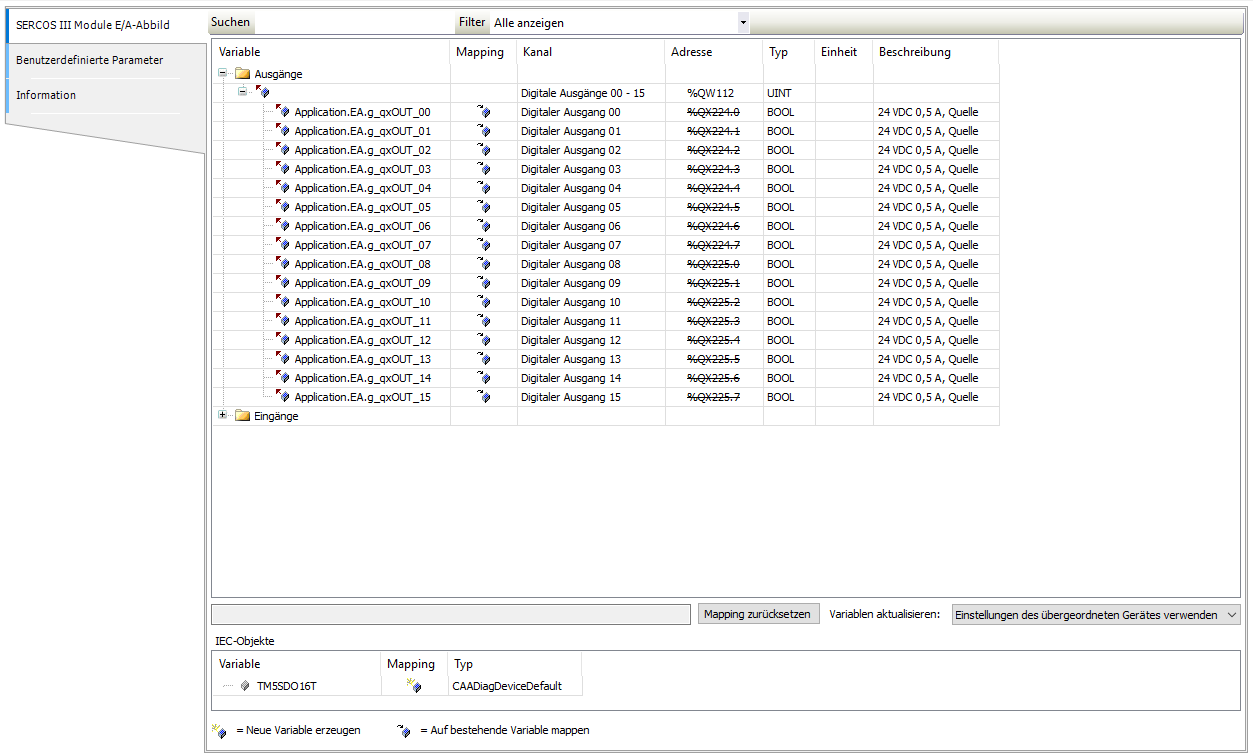
\includegraphics[width=.8\linewidth]{Images/TM5DO.PNG}%
            }
            \captionof{figure}{Zuweisung der digitalen Ausgänge des \small TM5SDO16T \normalsize Moduls}
            \label{fig:my-img27}
        \end{minipage}
    \end{enumerate}
    % Sichere Digitale Eingänge
    \item Zuweisung der sicheren digitalen Eingänge des Modicon \textit{TM5SDI4DFS} Modul:
    \begin{enumerate}
        \item Im Gerätebaum öffnen der Geräteeinstellungen des Moduls unter \textit{Sercos\_Master (Sercos Master)} ->\small \textit{BC\_TM5NS31 (BC\_TM5NS31)} -> \textit{TM5SDI4DFS}
        \item \normalsize Öffnen des Reiters \textit{TM5 Modul E/A-Abbild}
        \item \begin{minipage}[t]{\linewidth}
            \raggedright
            \adjustbox{valign=t}{%
                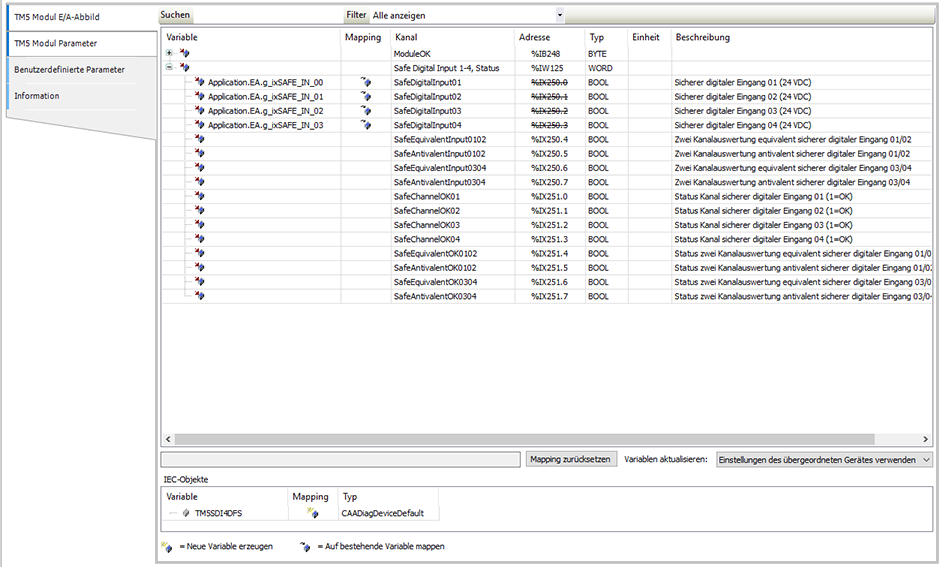
\includegraphics[width=.8\linewidth]{Images/TM5SDI.PNG}%
            }
            \captionof{figure}{Zuweisung der sicheren digitalen Eingänge des \small TM5SDI4DFS \normalsize Moduls}
            \label{fig:my-img28}
        \end{minipage}
    \end{enumerate}
    % Sichere Digitale Ausgänge
    \item Zuweisung der sicheren digitalen Ausgänge des Modicon \textit{TM5SDO4TFS} Modul:
    \begin{enumerate}
        \item Im Gerätebaum öffnen der Geräteeinstellungen des Moduls unter \textit{Sercos\_Master (Sercos Master)} ->\small \textit{BC\_TM5NS31 (BC\_TM5NS31)} -> \textit{TM5SDO4TFS}
        \item \normalsize Öffnen des Reiters \textit{TM5 Modul E/A-Abbild}
        \item \begin{minipage}[t]{\linewidth}
            \raggedright
            \adjustbox{valign=t}{%
                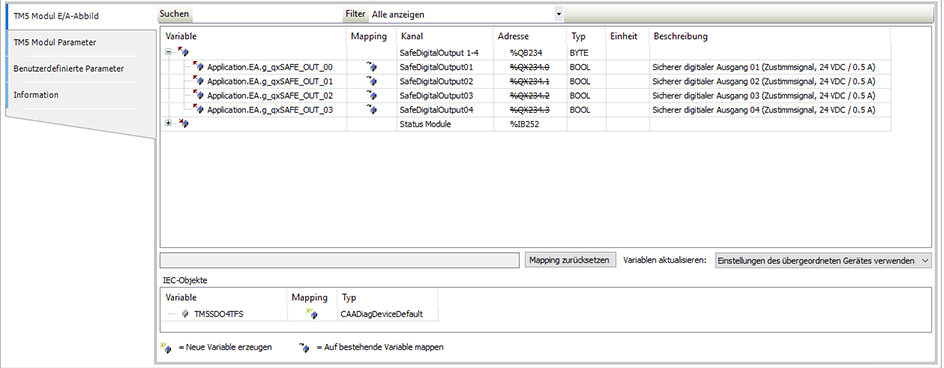
\includegraphics[width=.8\linewidth]{Images/TM5SDO.PNG}%
            }
            \captionof{figure}{Zuweisung der sicheren digitalen Ausgänge des \small TM5SDO4TFS \normalsize Moduls}
            \label{fig:my-img29}
        \end{minipage}
    \end{enumerate}
    % Analoge Eingänge
    \item Zuweisung der analogen Eingänge des Modicon \textit{TM5SAI4L} Modul:
    \begin{enumerate}
        \item Im Gerätebaum öffnen der Geräteeinstellungen des Moduls unter \textit{Sercos\_Master (Sercos Master)} ->\small \textit{BC\_TM5NS31 (BC\_TM5NS31)} -> \textit{TM5SAI4L}
        \item \normalsize Öffnen des Reiters \textit{TM5 Module E/A-Abbild}
        \item \begin{minipage}[t]{\linewidth}
            \raggedright
            \adjustbox{valign=t}{%
                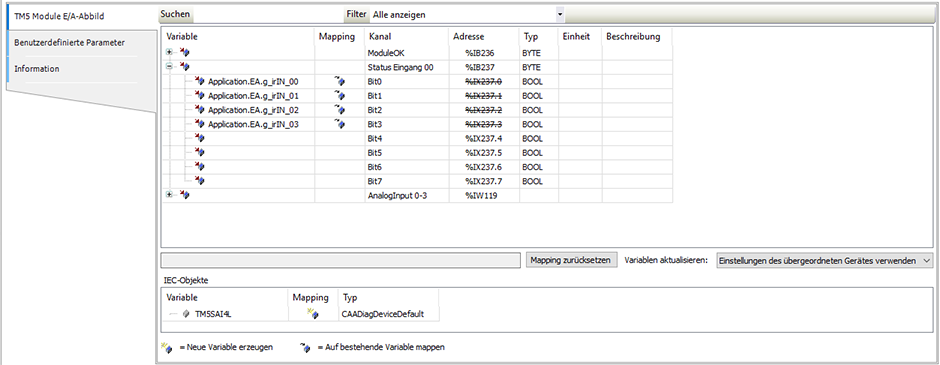
\includegraphics[width=.8\linewidth]{Images/TM5AI.PNG}%
            }
            \captionof{figure}{Zuweisung der analogen Eingänge des \small TM5SAI4L \normalsize Moduls}
            \label{fig:my-img30}
        \end{minipage}
    \end{enumerate}
    % Analoge Ausgänge
    \item Zuweisung der analogen Ausgänge des Modicon \textit{TM5SAO4L} Modul:
    \begin{enumerate}
        \item Im Gerätebaum öffnen der Geräteeinstellungen des Moduls unter \textit{Sercos\_Master (Sercos Master)} ->\small \textit{BC\_TM5NS31 (BC\_TM5NS31)} -> \textit{TM5SAO4L}
        \item \normalsize Öffnen des Reiters \textit{TM5 Module E/A-Abbild}
        \item \begin{minipage}[t]{\linewidth}
            \raggedright
            \adjustbox{valign=t}{%
                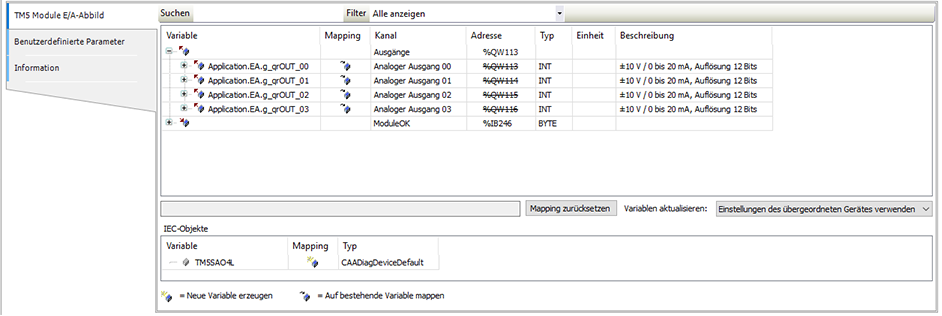
\includegraphics[width=.8\linewidth]{Images/TM5AO.PNG}%
            }
            \captionof{figure}{Zuweisung der analogen Ausgänge des \small TM5SAO4L \normalsize Moduls}
            \label{fig:my-img31}
        \end{minipage}
    \end{enumerate}
    % LMC <-> SLC E/A
    \item Zuweisung der Ein- \bzw Ausgänge der \textit{SLC\_TM5CSLC} Sicherheitssteuerung für den Datenaustausch mit dem \acs{lmc}:
    \begin{enumerate}
        \item Im Gerätebaum öffnen der Geräteeinstellungen der Sicherheitssteuerung unter \textit{Sercos\_Master (Sercos Master)} ->\small \textit{SLC\_TM5CSLCx00FS (SLC\_TM5CSLCx00FS)}
        \item \normalsize Öffnen des Reiters \textit{E/A-Abbild}
        \item \begin{minipage}[t]{\linewidth}
            \raggedright
            \adjustbox{valign=t}{%
                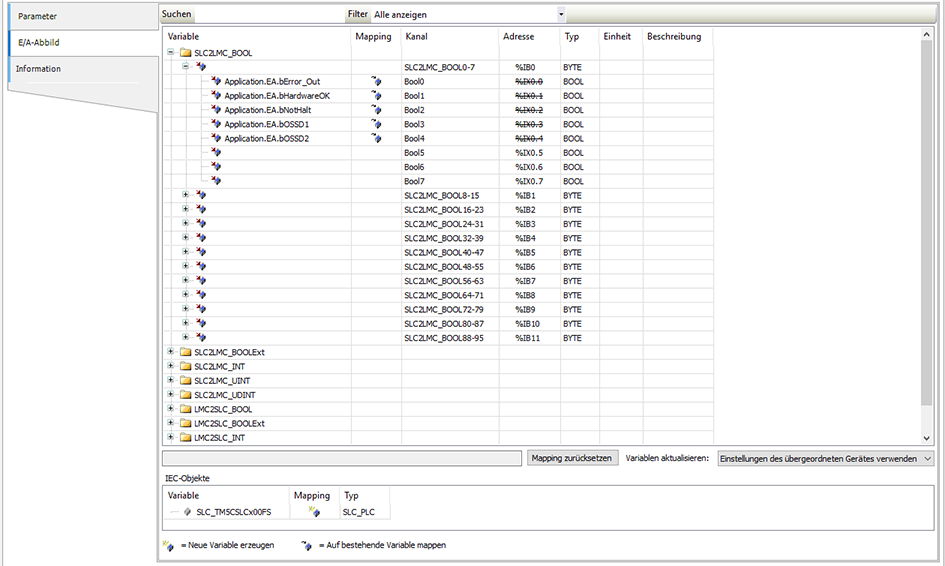
\includegraphics[width=.8\linewidth]{Images/SLC100.PNG}%
            }
            \captionof{figure}{Zuweisung der Variablen für den Datentransfer vom \acs{slc} zum \acs{lmc}}
            \label{fig:my-img32}
        \end{minipage}
        \item \begin{minipage}[t]{\linewidth}
            \raggedright
            \adjustbox{valign=t}{%
                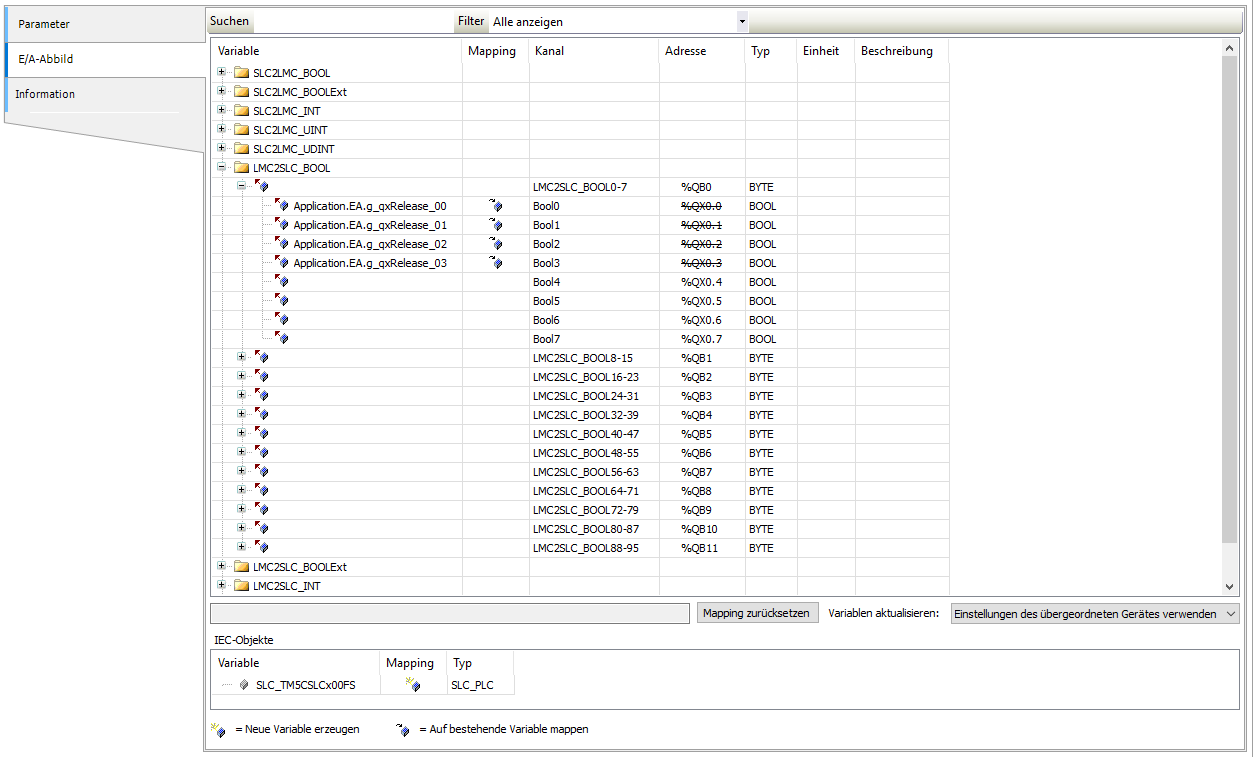
\includegraphics[width=.8\linewidth]{Images/SLC100_2.PNG}%
            }
            \captionof{figure}{Zuweisung der Variablen für den Datentransfer vom \acs{lmc} zum \acs{slc}}
            \label{fig:my-img33}
        \end{minipage}
    \end{enumerate}
\end{itemize}

Für die Nutzung der beiden Achsen des Systems muss die \textbf{Parametrierung und die Inbetriebnahme des Servoreglers} vorgenommen werden. Physisch gesehen handelt es sich zwar um ein Gerät, dass zwei Servoantriebe betreiben kann, in der Konfiguration im Programm werden die x-Achse und die z-Achse jedoch separat in Betrieb genommen. Die Parametrierung und die Inbetriebnahme erfolgt für beide Achsen Analog, da es sich bei beiden um die selben Motoren handelt, die in der selben Konfiguration genutzt werden.\\
Zunächst müssen einige physikalische Daten der beiden Achsen und deren zugehörigen Hardwarekomponenten in der Geräteparametrierung aufgenommen werden:

\begin{enumerate}
    \item Im Projektbaum öffnen der Datei \textit{Application} -> \textit{TemplateFullProgrammingFramework} -> \textit{EquipmentModules} -> \textit{SR\_BravoModule (PRG)} -> \textit{Init\_Slave1}
    \item Bis zum Kommentar \textit{***Manual***} scrollen (Zeile 171)
    \item \begin{minipage}[t]{\linewidth}
        \raggedright
        \adjustbox{valign=t}{%
            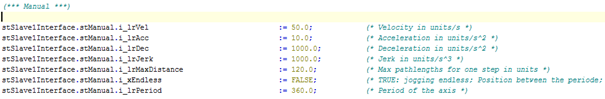
\includegraphics[width=.8\linewidth]{Images/Bewegungsparameter.png}%
        }
        \captionof{figure}{Einstellen der Bewegungsparameter für langsame manuelle Testfahrt}
        \label{fig:my-img34}
    \end{minipage}
    \bigskip \\
    rVel gibt die Geschwindigkeit in \si{mm/s} an, rAcc die Beschleunigung in \si{mm/s^2} und rDec die negative Beschleunigung \si{mm/s^2}.
    \item Im Projektbaum öffnen der Gerätedatei \textit{Sercos\_Master (Sercos Master)} -> \\ \textit{DRV\_Slave1}
    \item \begin{minipage}[t]{\linewidth}
        \raggedright
        \adjustbox{valign=t}{%
            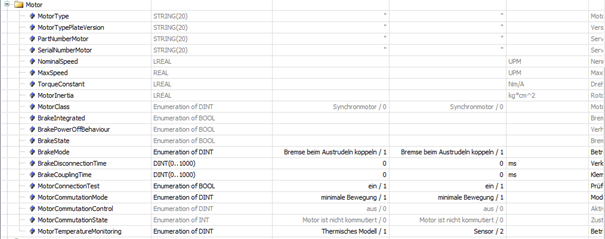
\includegraphics[width=.8\linewidth]{Images/Motorparametrierung.png}%
        }
        \captionof{figure}{Parametrierung des Motors für die x-Achse}
        \label{fig:my-img35}
    \end{minipage}
    \bigskip \\
    Der Wert \textit{MotorTemperatureMonitoring} wurde zur Temperaturüberwachung des Servomotors auf \textit{Thermisches Modell} gesetzt.
    \item \begin{minipage}[t]{\linewidth}
        \raggedright
        \adjustbox{valign=t}{%
            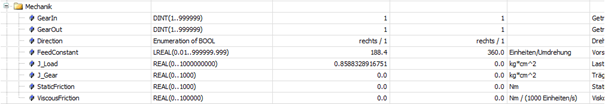
\includegraphics[width=.8\linewidth]{Images/Mechanikparametrierung.png}%
        }
        \captionof{figure}{Parametrierung der Machanik für die x-Achse}
        \label{fig:my-img36}
    \end{minipage}
    \bigskip \\
    Der Wert \textit{Direction} gibt den Drehsinn des Servomotors an. Die Einstellung \textit{rechts / 1} bedeutet, dass bei der Bedienung des Motors über die Steuerungsvisualisierung die Eingabe \textit{Jog+} zu einer Bewegungs der Achse nach links führt. Der Wert \textit{FeederConstant} muss selbst berechnet werden aus dem Motordurchmesser (\si{pi*M60mm}). Der \textit{JLoad} Wert gibt das Lastenträgheitsmoment in \si{kg*cm^2} an. Der einzusetzende Wert kann über die Software \textit{Machine Expert MotionBuilder} bestimmt werden. 
\end{enumerate}

Die gleichen Schritte müssen für die z-Achse analog zu der obigen Beschreibung durchgeführt werden.\\
\bigskip
Für den sicheren Betrieb der Achsen ist es erforderlich im \textit{MotionTemplateFull} Programmänderungen vorzunehmen, damit die Achsen bei den Endlagesensoren des Positioniersystems stoppen und nicht darüber hinaus bewegt werden können. Folgende Schritte sind dazu nötig:

\begin{enumerate}
    \item Im Projektbaum öffnen der Datei \textit{Application} -> \textit{TemplateFullProgrammingFramework} -> \textit{EquipmentModules} -> \textit{SR\_BravoModule (PRG)} -> \textit{SubModules\_Action}
    \item Bis zum Abschnitt 3 Scrollen und diesen auskommentieren oder löschen
    \item Abschnitt 4 (beinhaltet den Funktionsbaustein und Variablenzuweisungen für den \textit{DRV\_Slave2} \bzw die z-Achse) kopieren und wieder einfügen (duplizieren)
    \item Die Kopie editieren, so dass an jeder Stelle, wo \textit{DRV\_Slave2} aufgeführt ist nun \textit{DRV\_Slave1} steht
    \item \begin{minipage}[t]{\linewidth}
        \raggedright
        \adjustbox{valign=t}{%
            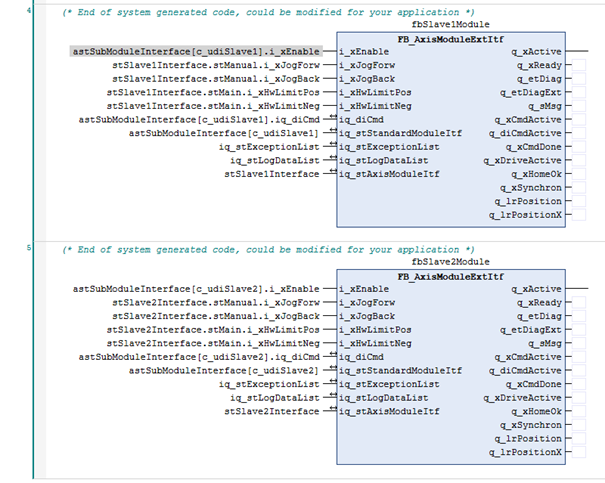
\includegraphics[width=.8\linewidth]{Images/Endlagesensoren.png}%
            % Hier muss ein Screenshot mit den richtigen Globalen Variablen eingefügt werden !!!
        }
        \captionof{figure}{Einbinden der Endlagesensoren}
        \label{fig:my-img37}
    \end{minipage}
    \bigskip \\
    Sowohl für den \textit{DRV\_Slave1} als auch den \textit{DRV\_Slave2} die globalen Variablen für die Endlagesensoren an den Stellen \textit{i\_xHwLimitPos} \bzw \textit{i\_xHwLimitNeg} einsetzen.
\end{enumerate}

Im nächsten Schritt wird die \textbf{Parametrierung und Inbetriebnahme des Netzteils} durchgeführt. Dafür muss zunächst wieder eine Hardwareparametrierung nach folgenden Schritten vorgenommen werden:

\begin{enumerate}
    \item Im Projektbaum öffnen der Gerätedatei \textit{Sercos\_Master (Sercos Master)} -> \\ \textit{PSM\_PowerSupply}
    \item \begin{minipage}[t]{\linewidth}
        \raggedright
        \adjustbox{valign=t}{%
            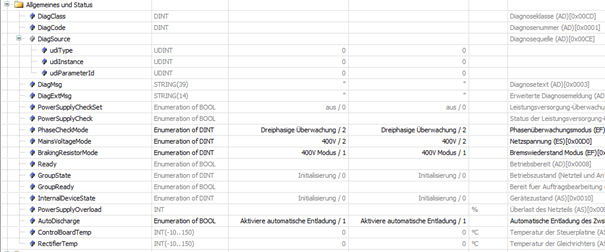
\includegraphics[width=.8\linewidth]{Images/Netzteilparameter.png}%
        }
        \captionof{figure}{Konfiguration des Netzteils}
        \label{fig:my-img38}
    \end{minipage}
    \bigskip \\
    Der \textit{PhaseCheckerMode} muss auf \textit{Dreiphasige Überwachung / 2} eingestellt werden, da das Netzteil dreiphasig angeschlossen und genutzt wird. Der \textit{MainsVoltageMode} wird gesetzt auf \textit{400\si{V} / 2} und der \textit{BrakingResistorMode} wird ebenfalls gesetzt auf \textit{400\si{V} Modus / 1}. Diese Werte ergeben sich ebenfalls aus dem dreiphasigen Anschluss des Netzteils.
\end{enumerate}

Je nachdem, ob bei der Verdrahtung ein Netzschütz verbaut oder diese weggelassen wurde, müssen nun weitere Programmänderungen am \textit{MotionTemplateFull} vorgenommen werden. An erster Stelle wird erklärt, wie ohne ein Netzschütz vorgegangen werden muss:

\begin{enumerate}
    \item Im Projektbaum öffnen der Datei \textit{Application} -> \textit{TemplateFullProgrammingFramework} -> \textit{TaskCalls} -> \textit{SR\_MainMachine (PRG)} -> \textit{Input\_Action}
    \item \begin{minipage}[t]{\linewidth}
        \raggedright
        \adjustbox{valign=t}{%
            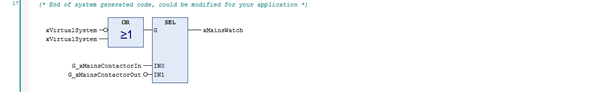
\includegraphics[width=\linewidth]{Images/MainsWatch.png}%
        }
        \captionof{figure}{Deaktivierung der Netzüberwachung}
        \label{fig:my-img39}
    \end{minipage}
    \bigskip \\
    Das Netzwerk in Abschnitt 17 muss erweitert werden um einen \textit{OR-Funktionsbaustein}, zu dem die Eingangsvariable \textit{xVirtualSystem} einmal negiert und einmal nicht-negiert zugewiesen wird. Diese Änderung deaktiviert die Netzüberwachung. Grundsätzlich sollte dieser Weg nicht gewählt und ein Netzschütz verbaut werden. 
\end{enumerate}

Bei der Verwendung eines Netzschützes sollte wie folgt vorgegangen werden:

\begin{enumerate}
    \item Mappen der Eingangsvariablen am LMC für die Netzschützrückmeldung
    \item Im Projektbaum öffnen der Datei \textit{Application} -> \textit{TemplateFullProgrammingFramework} -> \textit{TaskCalls} -> \textit{SR\_MainMachine (PRG)} -> \textit{Input\_Action}
    \item Zuweisen der Globalen Variablen für \textit{G\_xMainsContactorIn} und \\ \textit{G\_xMainsContactorOut}
\end{enumerate}

Im nächsten Schritt der Software-Implementation findet die \textbf{Implementation der funktionalen Sicherheit} statt. Dazu wird zunächst der Safety Logic Controller (\acs{slc}) konfiguriert:

\begin{enumerate}
    \item Im Projektbaum öffnen der Gerätedatei \textit{Sercos\_Master (Sercos Master)} -> \\ \textit{SLC\_TM5CSLCx00FS (TM5CSLCx00FS)}
    \item \begin{minipage}[t]{\linewidth}
        \raggedright
        \adjustbox{valign=t}{%
            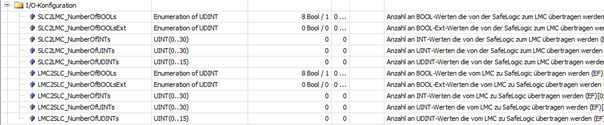
\includegraphics[width=\linewidth]{Images/SLCParameter.png}%
        }
        \captionof{figure}{I/O-Konfiguration des \acs{slc}}
        \label{fig:my-img40}
    \end{minipage}
    \bigskip \\
    Der Wert \textit{SLC2LMC\_NumberOFBOOLs} muss auf \textit{8 Bool / 1} gesetzt werden, sodass bis zu 8 Bool Werte vom Safety Logic Controller an den \acs{lmc} übertragen werden können. Analog muss der Wert \textit{LMC2SLC\_NumberOfBOOLs} auf \textit{8 Bool / 1} gesetzt werden, dass bis zu 8 Bool Werte vom \acs{LMC} an den \acs{SLC} gesendet werden können.
    \item Mapping der der neu verfügbaren \acs{ea}-Variablen von \bzw zu dem \acs{slc} (siehe \autoref{fig:my-img32} und \autoref{fig:my-img33})
\end{enumerate}

Anschließend kann das Programm für die Software-Implementation der funktionalen Sicherheit geschrieben werden. Dazu wird wie folgt vorgegangen:

\begin{enumerate}
    \item Im Projektbaum REchtsklick auf \textit{Sercos\_Master (Sercos Master)} -> \\ \textit{SLC\_TM5CSLCx00FS (TM5CSLCx00FS)}
    \item Im sich geöffneten Menü den Punkt \textit{SoSafe} -> \textit{SoSafe Programmable starten} auswählen
    \item Zunächst muss sowohl ein Passwort für die Entwicklung und die Inbetriebnahme des Sicherheitsprogramms festgelegt werden. Im der Arbeit beigefügten Programm ist das Passwort \text{admin1} für sowohl die Entwicklung als auch die Inbetriebnahme.
    \item Es müssen im sich nun geöffneten Dialogfenster alle Module (drei Module) per Chechbox ausgewählt werden
    \item Nun kann mit der Programmierung der Sicherheitsfunktionalitäten begonnen werden in der Funktionsbausteinsprache (FUP) nach IEC 61131-3
    \item \begin{minipage}[t]{\linewidth}
        \raggedright
        \adjustbox{valign=t}{%
            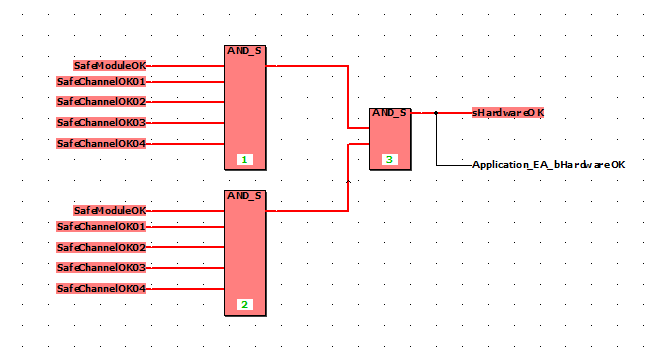
\includegraphics[width=.7\linewidth]{Images/SoSafe1.PNG}%
        }
        \captionof{figure}{Hardwareprüfung der sicheren \acs{ea}-Module}
        \label{fig:my-img41}
    \end{minipage}
    \bigskip \\
    Die sichere Variable \textit{sHardwareOK} wird auf den Wert \textbf{TRUE} gesetzt, wenn sowohl die beiden \acs{ea}-Module keine Hardwarefehler aufweisen und die Verdrahtung der Eingänge und Ausgänge korrekt ist. Weiterhin wird der Wert über die Variable \textit{Application\_EA\_bHardwareOK} auch an den \acs{lmc} weitergeleitet, um im Hauptprogramm genutzt zu werden (\zB für die Ausgabe über OPC UA).
    \item \begin{minipage}[t]{\linewidth}
        \raggedright
        \adjustbox{valign=t}{%
            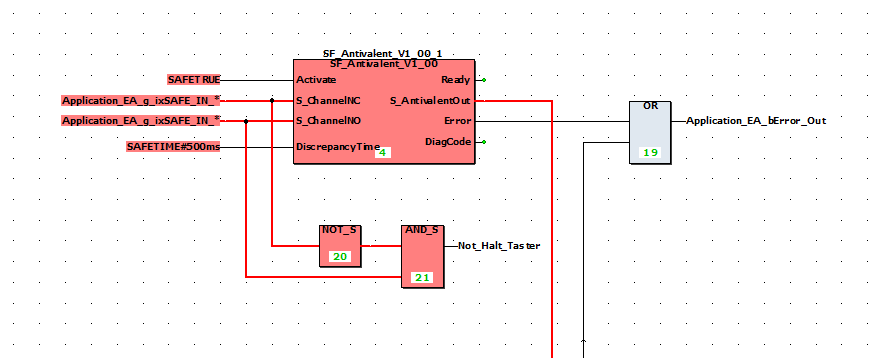
\includegraphics[width=\linewidth]{Images/SoSafe2.PNG}%
        }
        \captionof{figure}{Sicherer SF\_Antivalent Funktionbaustein für die Verarbeitung der Not-Halt-Auslösung}
        \label{fig:my-img42}
    \end{minipage}
    \bigskip \\
    Bei dem sicheren Funktionsbaustein \textit{SF\_Antivalent\_V1\_00\_1} handelt es sich um einen Baustein, der die beiden Antivalenten Eingänge für die Not-Halt-Taster Auslösung verarbeitet. Ist die Variable \textit{Application\_EA\_g\_ixSafe\_IN\_01} \textbf{FALSE} und die Variable \textit{Application\_EA\_g\_ixSafe\_IN\_00} \textbf{TRUE}, so schaltet der Ausgang \textit{S\_AntivalentOut} auf \textbf{TRUE}. Der Wert des Ausgangs wird im nächsten Bild weiterverarbeitet. Für die Weitergabe des Gleichen Wertes an den \acs{lmc} wird der Baustein nicht benötigt und die beiden Eingänge können per \textit{AND\_S}-Baustein verundet werden (unter Berücksichtigung, dass der Eingang \textit{Application\_EA\_g\_ixSafe\_IN\_01} negiert werden muss). Der \textit{Error} Ausgang kann auch verbunden und die Information an den \acs{lmc} weitergegeben werden in der Variable \textit{Application\_EA\_bError\_Out}.
    \item \begin{minipage}[t]{\linewidth}
        \raggedright
        \adjustbox{valign=t}{%
            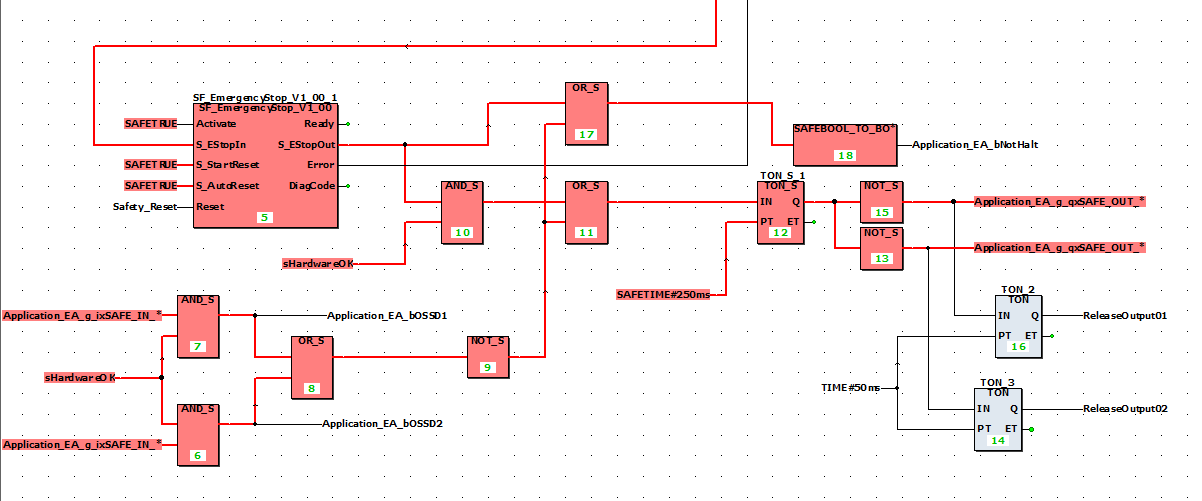
\includegraphics[width=\linewidth]{Images/SoSafe3.PNG}%
        }
        \captionof{figure}{Verarbeitung des Not-Halt-Signals und der Lichtvorhangssignale}
        \label{fig:my-img43}
    \end{minipage}
    \item Zunächst wird der sichere Funktionsbaustein \textit{SF\_EmergencyStop\_V1\_00\_1} hinzugefügt. In den Eingang \textit{S\_EStopIn} wird das Ausgangssignal des Antivalent-Funktionsbausteins gelegt. Wird der Not-Halt aktiviert, schaltet der Ausgang \\ \textit{S\_EStopOut} des Bausteins auf \textbf{TRUE}. Über den \textit{Reset}-Eingang muss der Baustein wieder Freigegeben werden, so dass der Ausgang wieder auf \textbf{FALSE} umschaltet. Auf den Reset-Eingang wird die Variable \textit{>Safety\_Reset} gelegt, die vom \acs{lmc} an den \acs{slc} weitergeleitet wird. Somit kann durch das Auslösen des Hardware Reset-Tasters am \acs{lmc} der Funktionsbaustein wieder freigegeben \bzw zurückgesetzt werden. Die Eingänge \textit{S\_StartReset} und \textit{S\_AutoReset} sollten auf \textbf{SAFEFALSE} gesetzt werden. Im Bild ist jedoch vorerst zu erkennen, dass die Werte auf \textbf{SAFETRUE} gesetzt sind, da zum Testen des Sicherheitsprogramms ein automatisches zurücksetzen das Drücken des Reset-Tasters hinfällig macht und somit Zeit spart.
    \item Anschließend werden die beiden sicheren Eingänge \textit{Application\_EA\_g\_ixSafe\_IN\_02} und \textit{Application\_EA\_g\_ixSafe\_IN\_03} verarbeitet. Dabei handelt es sich um den Lichtvorhang (OSSD1 und OSSD2). Die beiden Eingänge müssen jeweils verundet werden mit der Variable \textit{bHardwareOK}. Ist eines der beiden Signale des Lichtvorhangs \textbf{FALSE}, so muss der Ausgang, dessen Signal später mit dem Not-Halt-Signal verodert wird \textbf{TRUE} sein (umgesetzt durch ein \textit{S\_ODER}- und ein \textit{S\_Not}-Baustein).
    \item Wie bereits im vorherigen Schritt angedeutet wird nun das Ausgangssignal der LichtvorhangSchaltung mit dem Ausgang der Not-Halt-Schlatung verodert. Wichtig ist, dass das Not-Halt-Signal auch mit dem Wert der Variablen \textit{sHardwareOK} verundet wird, um Hardwarefehler auszuschließen.
    \item Im nächsten Schritt wird das Not-Halt-Signal zu einem nicht-sicheren Bool-Wert umgewandelt, welcher über die Variable \textit{Application\_EA\_bNotHalt} an den \acs{lmc} übergeben wird.
    \item Der letzte Schritt in der Programmierung des Sicherheitsprogrammes ist das setzen der Ausgänge des \acs{slc}. Wichtig ist zu beachten, dass die Ausgänge mit dem \textit{IverterEnable}-Eingang des Servoreglers (LXM 62D) verbunden sind. Nehmen die Ausgänge den Wert \textbf{FALSE} an, schaltet der Servoregler ab. Das soll dann passieren, wenn der Not-Halt ausgelöst \bzw der Lichtvorhang durchbrochen wurde. Jedoch ist es notwendig, dass die Motoren zunächst angehalten haben, bevor der Regler abgeschaltet wird, da sonst bei zu frühem Abschalten des Reglers der Bremsvorgang nicht fortgesetzt wird und die beiden Achsen des Positioniersystems austrudeln würden. Dies könnte dafür sorgen, dass die Schlitten auf den Achsen über die Endlagen hinausrutschen und Beschädigungen an der ANlage verursachen. Deshalb wird über ein \textit{S\_TON}-Baustein die Abschaltung der Ausgänge um 250\si{ms} verzögert. In \autoref{fig:my-img43} ist zu erkennen, dass zwei weitere nicht-sichere TONs genutzt wurden. Diese sind für das Lösen der Ausgänge nach einem Signalwechsel zuständig. Es handelt sich dabei um eine Sicherheitsmaßnahme, so das Ausgänge nach Wertänderung immer gesteuert wieder freigegeben werden.
\end{enumerate}

Nachdem nun das Sicherheitsprogramm komplettiert ist, kann die SoSafe Programmable Umgebung wieder verlassen werden. Abschließend muss eine letzte Änderung am \textit{MotionTemplateFull} vorgenommen werden, um den Not-Halt auch auf \acs{lmc}-Seite zu implementieren. Dazu sind folgende Schritte nötig:

\begin{enumerate}
    \item Im Projektbaum öffnen der Datei \textit{Application} -> \textit{TemplateFullProgrammingFramework} -> \textit{TaskCalls} -> \textit{SR\_HWCopyIO}
    \item \begin{minipage}[t]{\linewidth}
        \raggedright
        \adjustbox{valign=t}{%
            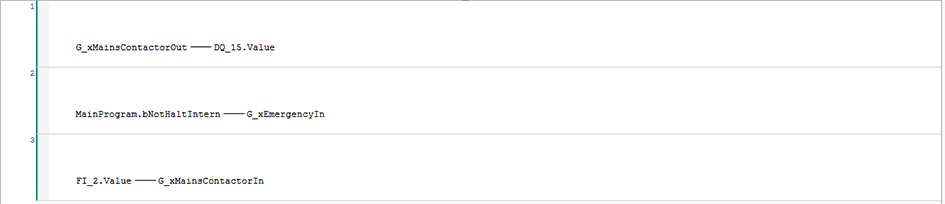
\includegraphics[width=\linewidth]{Images/NotHaltLMC.png}%
        }
        \captionof{figure}{Zuweisung der Not-Halt-Variable im \acs{lmc}}
        \label{fig:my-img44}
    \end{minipage}
    \bigskip \\
    Der internen Variable \textit{G\_xEmergencyIn} wird die Not-Halt-Ausgangsvariable aus dem \acs{slc} zugewiesen. Nun bekommt auch das \textit{MotionTemplateFull} das reale Not-Halt-Signal zur verfügung gestellt und kann dieses verarbeiten (\zB für den Software Not-Halt-Reset aus der Steuerungsvisualisierung).
\end{enumerate}

Der letzte Schritt der Software Implementation ist die Einrichtung des \acs{lmc}400c asowie der Wago Wago PFC200 Steuerung für die Nutzung als OPC UA Server. Dabei sind die SChritte für beide Steuerungen identisch. Es unterscheiden sich jediglich die Daten, die über OPC kommuniziert werden können. Der \acs{lmc} soll vor allem Positionsdaten und für die Positionierung relevante Daten bereitstellen können, als auch lesen. Die Wago Steuerung ist verantwortlich für die Messung von Verbrauchswerten des Systems, wie der benmötigte Strom oder die Leistungsaufnahme. Diese Daten werden über den Wago OPC Server bereitgestellt. Für die Implementierung der OPC Funktionalität werden auf beiden Steuerungen folgende Schritte durchgeführt:

\begin{enumerate}
    \item Es wird eine weitere globale Variablenliste angelegt, die alle Variablen enthält, die per OPC versendet \bzw empfangen werden sollen.
    \item Im Hauptprogramm werden die globalen Variablen mit den Werten der relevanten Variablen im PRogramm gefüllt.
    \item Im nächsten Schritt wird eine Symbolkonfiguration angelegt unter beachtung der Auswahl der Checkbox für die OPC Kompatibilität.
    \item Zunächst wird die Symbolkonfiguration einmal gebaut per Button in der oberen Leiste.
    \item Anschließend wird die neu erstellte Variablenliste per Haken selektiert.
    \item Nach erneutem Bauen und der Übertragung an des Programmes ist die OPC Kommunikation betriebsbereit
\end{enumerate}

Mit Fertigstellung der Software-Implementation der funktionalen sicherheit ist die Implementierung sämtlicher Modelle aus der Projektierungs- \bzw Modellierungsphase abgeschlossen. Anschließend gilt es die Anforderungen an das System mit Hilfe der Testkriterien zu diesen zu überprüfen, um sicherzustellen, dass die nun implementierten Funktionalitäten die Anforderungen erfüllen.

\end{document}